\documentclass[11pt,a4paper]{article}

\usepackage[T1]{fontenc}
\usepackage{lmodern}
\usepackage[a4paper,margin=18mm,top=20mm,bottom=19mm,headheight=22pt]{geometry}
\usepackage{amsmath,amssymb,mathtools,bm}
\usepackage{booktabs,tabularx,array,multicol}
\usepackage{enumitem}
\usepackage[most]{tcolorbox}
\usepackage{xcolor}
\usepackage{titlesec}
\usepackage{fancyhdr}
\usepackage{hyperref}
\usepackage{microtype}
\usepackage{tikz}
\usepackage{pgfplots}
\pgfplotsset{compat=1.18}
\usetikzlibrary{arrows.meta,calc,positioning,fit,backgrounds,matrix,patterns,decorations.pathreplacing}

\definecolor{Navy}{HTML}{173B57}
\definecolor{Blue}{HTML}{2D6A9F}
\definecolor{Teal}{HTML}{177C76}
\definecolor{Orange}{HTML}{B9652B}
\definecolor{Red}{HTML}{A43D3D}
\definecolor{Ink}{HTML}{26343D}
\definecolor{Muted}{HTML}{66757F}
\definecolor{PaleBlue}{HTML}{F1F6FA}
\definecolor{PaleTeal}{HTML}{EFF8F6}
\definecolor{PaleOrange}{HTML}{FFF7EF}
\definecolor{PaleRed}{HTML}{FFF2F2}
\definecolor{Rule}{HTML}{CBD7DF}

\hypersetup{
  colorlinks=true,
  linkcolor=Navy,
  urlcolor=Blue,
  citecolor=Teal,
  pdftitle={CS3244 Machine Learning Notes},
  pdfauthor={},
  pdfsubject={CS3244 machine learning study notes}
}

\pagestyle{fancy}
\fancyhf{}
\fancyhead[L]{\small\color{Navy}\textbf{CS3244} Machine Learning}
\fancyhead[R]{\small\color{Muted}Study Notes}
\fancyfoot[L]{\scriptsize\color{Muted}\texttt{Gao327}}
\fancyfoot[C]{\scriptsize\color{Muted}Unofficial study material; current course materials remain authoritative}
\fancyfoot[R]{\small\color{Ink}\thepage}
\renewcommand{\headrulewidth}{0.4pt}
\renewcommand{\headrule}{\hbox to\headwidth{\color{Rule}\leaders\hrule height \headrulewidth\hfill}}

\setlength{\parindent}{2em}
\setlength{\parskip}{2.2pt}
\setlist[itemize]{leftmargin=1.55em,itemsep=2pt,topsep=3pt}
\setlist[enumerate]{leftmargin=1.8em,itemsep=2pt,topsep=3pt}
\renewcommand{\arraystretch}{1.17}
\newcolumntype{Y}{>{\raggedright\arraybackslash}X}
\allowdisplaybreaks[2]

\titleformat{\section}
  {\Large\bfseries\color{Navy}}{\thesection}{0.65em}{}
\titleformat{\subsection}
  {\large\bfseries\color{Blue}}{\thesubsection}{0.55em}{}
\titleformat{\subsubsection}
  {\normalsize\bfseries\color{Teal}}{\thesubsubsection}{0.5em}{}

\newtcolorbox{definition}[1][]{
  enhanced,breakable,colback=PaleBlue,colframe=Blue,
  boxrule=0.6pt,arc=1.5mm,left=2.5mm,right=2.5mm,top=1.6mm,bottom=1.6mm,
  fonttitle=\bfseries,title={#1}
}
\newtcolorbox{derivation}[1][]{
  enhanced,breakable,colback=PaleTeal,colframe=Teal,
  boxrule=0.6pt,arc=1.5mm,left=2.5mm,right=2.5mm,top=1.6mm,bottom=1.6mm,
  fonttitle=\bfseries,title={#1}
}
\newtcolorbox{condition}[1][]{
  enhanced,breakable,colback=PaleOrange,colframe=Orange,
  boxrule=0.6pt,arc=1.5mm,left=2.5mm,right=2.5mm,top=1.6mm,bottom=1.6mm,
  fonttitle=\bfseries,title={#1}
}
\newtcolorbox{correction}[1][]{
  enhanced,breakable,colback=PaleRed,colframe=Red,
  boxrule=0.6pt,arc=1.5mm,left=2.5mm,right=2.5mm,top=1.6mm,bottom=1.6mm,
  fonttitle=\bfseries,title={#1}
}
\newtcolorbox{examplebox}[1][]{
  enhanced,breakable,colback=white,colframe=Rule,
  boxrule=0.6pt,arc=1.5mm,left=2.5mm,right=2.5mm,top=1.6mm,bottom=1.6mm,
  fonttitle=\bfseries,title={#1}
}

\newcommand{\R}{\mathbb{R}}
\newcommand{\E}{\mathbb{E}}
\newcommand{\Prob}{\mathbb{P}}
\newcommand{\Var}{\operatorname{Var}}
\newcommand{\Cov}{\operatorname{Cov}}
\newcommand{\argmin}{\operatorname*{arg\,min}}
\newcommand{\argmax}{\operatorname*{arg\,max}}
\newcommand{\sign}{\operatorname{sign}}
\newcommand{\softmax}{\operatorname{softmax}}
\newcommand{\diag}{\operatorname{diag}}
\newcommand{\tr}{\operatorname{tr}}
\newcommand{\norm}[1]{\left\lVert #1\right\rVert}
\newcommand{\abs}[1]{\left\lvert #1\right\rvert}
\newcommand{\inner}[2]{\left\langle #1,#2\right\rangle}
\newcommand{\vect}[1]{\bm{#1}}
\newcommand{\ind}{\mathbb{I}}
\newcommand{\dd}{\,\mathrm{d}}

% Editable vector figures used throughout the notes.

\newcommand{\TrainingPipelineFigure}{%
\begin{figure}[htbp]
\centering
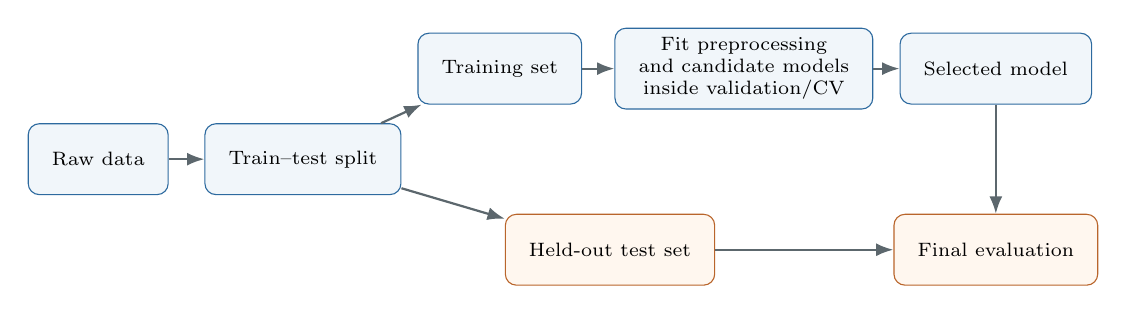
\begin{tikzpicture}[
  box/.style={draw=Blue,rounded corners,fill=PaleBlue,align=center,minimum height=9mm,inner xsep=3mm,font=\scriptsize},
  held/.style={draw=Orange,rounded corners,fill=PaleOrange,align=center,minimum height=9mm,inner xsep=3mm,font=\scriptsize},
  arr/.style={-{Latex[length=2.2mm]},thick,color=Ink!75}
]
\node[box] (data) at (0,0) {Raw data};
\node[box] (split) at (2.6,0) {Train--test split};
\node[box] (train) at (5.1,1.15) {Training set};
\node[box] (prep) at (8.2,1.15) {Fit preprocessing\\and candidate models\\inside validation/CV};
\node[box] (model) at (11.4,1.15) {Selected model};
\node[held] (test) at (6.5,-1.15) {Held-out test set};
\node[held] (report) at (11.4,-1.15) {Final evaluation};
\draw[arr] (data) -- (split);
\draw[arr] (split) -- (train);
\draw[arr] (train) -- (prep);
\draw[arr] (prep) -- (model);
\draw[arr] (split) -- (test);
\draw[arr] (model) -- (report);
\draw[arr] (test) -- (report);
\end{tikzpicture}
\caption{Information boundaries in a training workflow. Scaling, feature selection, and resampling are fitted only on training data or training folds. The test set is used once, after model selection.}
\label{fig:training-pipeline}
\end{figure}}

\newcommand{\KnnGeometryFigure}{%
\begin{figure}[htbp]
\centering
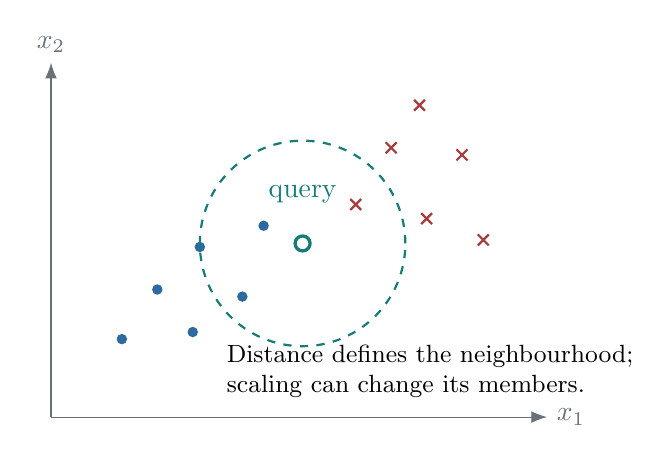
\begin{tikzpicture}[scale=0.9]
\draw[-{Latex[length=2mm]},color=Ink!70] (0,0) -- (7,0) node[right] {$x_1$};
\draw[-{Latex[length=2mm]},color=Ink!70] (0,0) -- (0,5) node[above] {$x_2$};
\foreach \p in {(1.0,1.1),(1.5,1.8),(2.0,1.2),(2.1,2.4),(2.7,1.7),(3.0,2.7)}
  \fill[Blue] \p circle (2.1pt);
\foreach \p in {(4.3,3.0),(4.8,3.8),(5.3,2.8),(5.8,3.7),(6.1,2.5),(5.2,4.4)}
  \draw[Red,thick] \p ++(-2.2pt,-2.2pt) -- ++(4.4pt,4.4pt) \p ++(-2.2pt,2.2pt) -- ++(4.4pt,-4.4pt);
\coordinate (q) at (3.55,2.45);
\draw[Teal,very thick] (q) circle (3pt);
\draw[Teal,dashed,thick] (q) circle (1.45cm);
\node[Teal] at (3.55,3.15) {query};
\node[font=\small,align=left] at (5.35,0.65) {Distance defines the neighbourhood;\\scaling can change its members.};
\end{tikzpicture}
\caption{KNN searches for $k$ observations around a query. The circle represents one neighbourhood under a chosen distance scale; neighbourhoods become sparse in high dimensions.}
\label{fig:knn-geometry}
\end{figure}}

\newcommand{\LinearMarginFigure}{%
\begin{figure}[htbp]
\centering
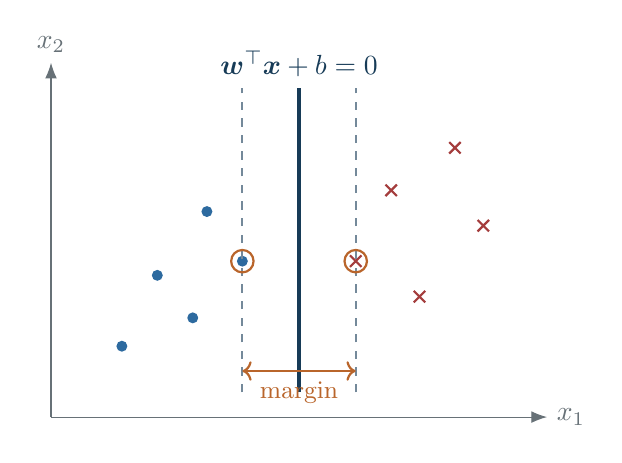
\begin{tikzpicture}[scale=0.9]
\draw[-{Latex[length=2mm]},color=Ink!70] (0,0) -- (7,0) node[right] {$x_1$};
\draw[-{Latex[length=2mm]},color=Ink!70] (0,0) -- (0,5) node[above] {$x_2$};
\foreach \p in {(1.0,1.0),(1.5,2.0),(2.0,1.4),(2.2,2.9),(2.7,2.2)}
  \fill[Blue] \p circle (2.2pt);
\foreach \p in {(4.3,2.2),(4.8,3.2),(5.2,1.7),(5.7,3.8),(6.1,2.7)}
  \draw[Red,thick] \p ++(-2.3pt,-2.3pt) -- ++(4.6pt,4.6pt) \p ++(-2.3pt,2.3pt) -- ++(4.6pt,-4.6pt);
\draw[Navy,very thick] (3.5,0.35) -- (3.5,4.65) node[above] {$\vect w^\top\vect x+b=0$};
\draw[Navy!60,dashed,thick] (2.7,0.35) -- (2.7,4.65);
\draw[Navy!60,dashed,thick] (4.3,0.35) -- (4.3,4.65);
\draw[<->,Orange,thick] (2.7,0.65) -- node[below,font=\small] {margin} (4.3,0.65);
\draw[Orange,thick] (2.7,2.2) circle (4.5pt);
\draw[Orange,thick] (4.3,2.2) circle (4.5pt);
\end{tikzpicture}
\caption{Logistic regression, the perceptron, and SVM use the same linear score $z=\vect w^\top\vect x+b$. SVM additionally chooses a boundary with maximum geometric margin.}
\label{fig:linear-margin}
\end{figure}}

\newcommand{\BiasVarianceFigure}{%
\begin{figure}[htbp]
\centering
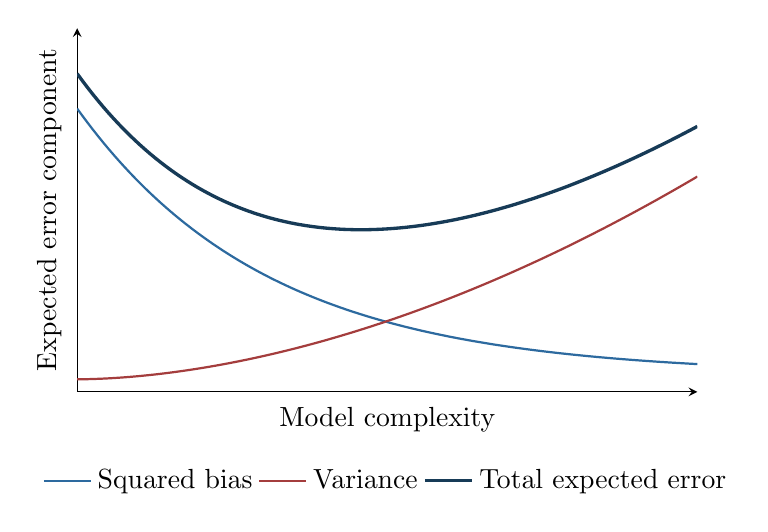
\begin{tikzpicture}
\begin{axis}[
  width=0.78\textwidth,height=6.2cm,
  axis lines=left,xlabel={Model complexity},ylabel={Expected error component},
  xmin=0,xmax=5,ymin=0,ymax=5.2,
  xtick=\empty,ytick=\empty,
  legend style={draw=none,fill=none,at={(0.5,-0.18)},anchor=north,legend columns=3},
  samples=120,domain=0:5
]
\addplot[Blue,thick] {3.8*exp(-0.65*x)+0.25};
\addlegendentry{Squared bias}
\addplot[Red,thick] {0.18+0.16*x^1.8};
\addlegendentry{Variance}
\addplot[Navy,very thick] {3.8*exp(-0.65*x)+0.16*x^1.8+0.75};
\addlegendentry{Total expected error}
\end{axis}
\end{tikzpicture}
\caption{As model complexity grows, bias often falls while variance rises. These curves describe a common pattern rather than a theorem for every model family; irreducible noise shifts the total error upward.}
\label{fig:bias-variance}
\end{figure}}

\newcommand{\PcaLdaFigure}{%
\begin{figure}[htbp]
\centering
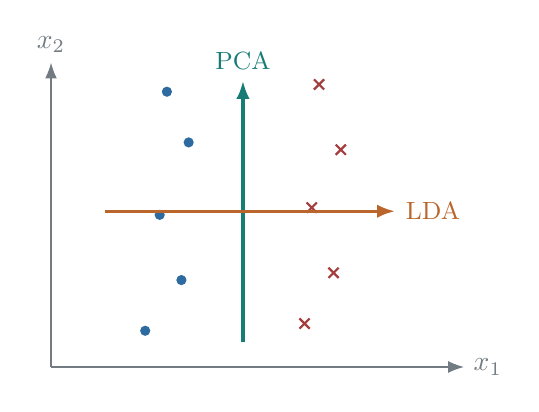
\begin{tikzpicture}[scale=0.92]
\begin{scope}
\draw[-{Latex[length=2mm]},color=Ink!65] (0,0)--(5.7,0) node[right] {$x_1$};
\draw[-{Latex[length=2mm]},color=Ink!65] (0,0)--(0,4.2) node[above] {$x_2$};
\foreach \p in {(1.3,0.5),(1.8,1.2),(1.5,2.1),(1.9,3.1),(1.6,3.8)} \fill[Blue] \p circle (2pt);
\foreach \p in {(3.5,0.6),(3.9,1.3),(3.6,2.2),(4.0,3.0),(3.7,3.9)}
  \draw[Red,thick] \p ++(-2pt,-2pt)--++(4pt,4pt) \p ++(-2pt,2pt)--++(4pt,-4pt);
\draw[Teal,very thick,-{Latex[length=2.3mm]}] (2.65,0.35)--(2.65,3.95) node[above,font=\small] {PCA};
\draw[Orange,very thick,-{Latex[length=2.3mm]}] (0.75,2.15)--(4.75,2.15) node[right,font=\small] {LDA};
\end{scope}
\end{tikzpicture}
\caption{PCA selects directions of high total variance. LDA selects directions that maximise the ratio of between-class to within-class scatter. Their objectives are different.}
\label{fig:pca-lda}
\end{figure}}

\newcommand{\BackpropFigure}{%
\begin{figure}[htbp]
\centering
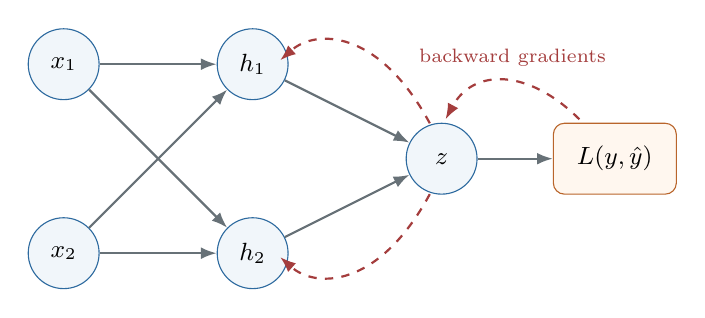
\begin{tikzpicture}[
  neuron/.style={circle,draw=Blue,fill=PaleBlue,minimum size=9mm,font=\small},
  loss/.style={rounded corners,draw=Orange,fill=PaleOrange,minimum height=9mm,inner xsep=3mm,font=\small},
  fwd/.style={-{Latex[length=2mm]},thick,color=Ink!70},
  bwd/.style={-{Latex[length=2mm]},thick,color=Red,dashed}
]
\node[neuron] (x1) at (0,1.2) {$x_1$};
\node[neuron] (x2) at (0,-1.2) {$x_2$};
\node[neuron] (h1) at (2.4,1.2) {$h_1$};
\node[neuron] (h2) at (2.4,-1.2) {$h_2$};
\node[neuron] (z) at (4.8,0) {$z$};
\node[loss] (l) at (7.0,0) {$L(y,\hat y)$};
\foreach \a in {x1,x2}\foreach \b in {h1,h2}\draw[fwd] (\a)--(\b);
\draw[fwd] (h1)--(z); \draw[fwd] (h2)--(z); \draw[fwd] (z)--(l);
\draw[bwd] (6.55,0.5) .. controls (5.9,1.15) and (5.2,1.15) .. (4.85,0.5);
\draw[bwd] (4.65,0.45) .. controls (4.0,1.65) and (3.2,1.65) .. (2.75,1.25);
\draw[bwd] (4.65,-0.45) .. controls (4.0,-1.65) and (3.2,-1.65) .. (2.75,-1.25);
\node[Red,font=\scriptsize] at (5.7,1.28) {backward gradients};
\end{tikzpicture}
\caption{Backpropagation starts at the loss and applies the chain rule along the reversed computation graph. Activations stored during the forward pass are reused to obtain parameter gradients.}
\label{fig:backprop}
\end{figure}}

\newcommand{\ArchitectureFigure}{%
\begin{figure}[htbp]
\centering
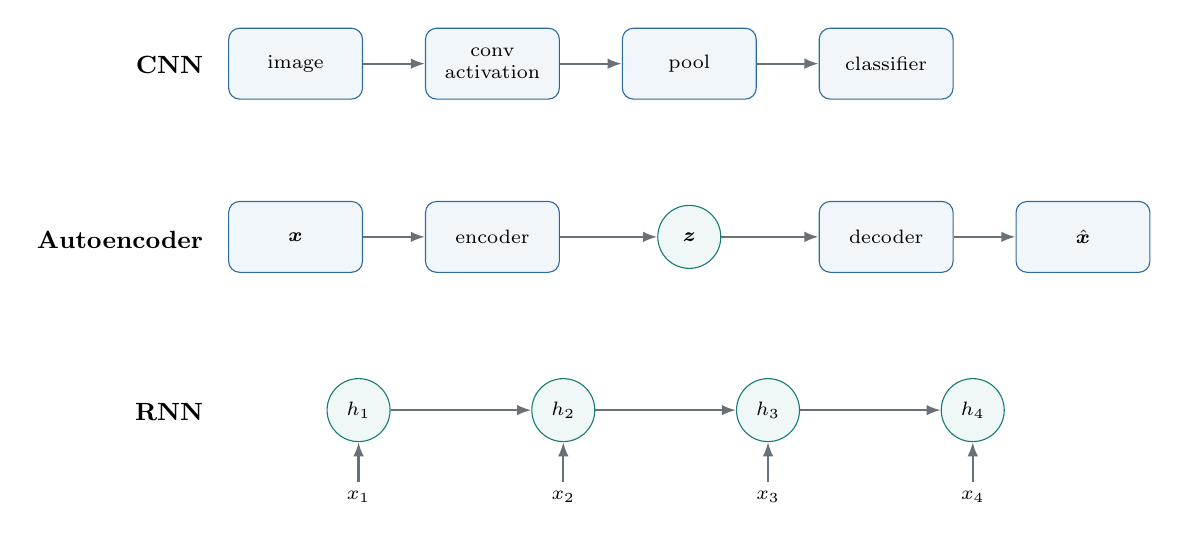
\begin{tikzpicture}[
  block/.style={draw=Blue,rounded corners,fill=PaleBlue,minimum width=17mm,minimum height=9mm,align=center,font=\scriptsize},
  state/.style={draw=Teal,circle,fill=PaleTeal,minimum size=8mm,font=\scriptsize},
  arr/.style={-{Latex[length=1.8mm]},thick,color=Ink!70}
]
\node[font=\bfseries\small,anchor=e] at (-1.05,2.2) {CNN};
\node[block] (im) at (0,2.2) {image};
\node[block] (cv) at (2.5,2.2) {conv\\activation};
\node[block] (pl) at (5.0,2.2) {pool};
\node[block] (cl) at (7.5,2.2) {classifier};
\draw[arr] (im)--(cv); \draw[arr] (cv)--(pl); \draw[arr] (pl)--(cl);

\node[font=\bfseries\small,anchor=e] at (-1.05,0) {Autoencoder};
\node[block] (aein) at (0,0) {$\vect x$};
\node[block] (enc) at (2.5,0) {encoder};
\node[state] (lat) at (5.0,0) {$\vect z$};
\node[block] (dec) at (7.5,0) {decoder};
\node[block] (aeout) at (10.0,0) {$\hat{\vect x}$};
\draw[arr] (aein)--(enc); \draw[arr] (enc)--(lat); \draw[arr] (lat)--(dec); \draw[arr] (dec)--(aeout);

\node[font=\bfseries\small,anchor=e] at (-1.05,-2.2) {RNN};
\foreach \i/\x in {1/0.8,2/3.4,3/6.0,4/8.6}{
  \node[state] (h\i) at (\x,-2.2) {$h_{\i}$};
  \node[font=\scriptsize,below=5mm of h\i] (x\i) {$x_{\i}$};
  \draw[arr] (x\i)--(h\i);
}
\draw[arr] (h1)--(h2); \draw[arr] (h2)--(h3); \draw[arr] (h3)--(h4);
\end{tikzpicture}
\caption{The architectures encode different assumptions: CNNs use spatial locality, RNNs share a state transition across time, and autoencoders learn a bottleneck through reconstruction.}
\label{fig:architectures}
\end{figure}}


\begin{document}

\begin{tcolorbox}[
  enhanced,colback=Navy,colframe=Navy,arc=2.5mm,boxrule=0pt,
  left=7mm,right=7mm,top=8mm,bottom=7mm
]
{\color{white}\fontsize{25}{29}\selectfont\bfseries CS3244 Machine Learning\par}
\vspace{2mm}
\end{tcolorbox}

\section*{Scope and notation}
\addcontentsline{toc}{section}{Scope and notation}

These notes develop the main ideas of machine learning from foundational statistical learning and classical models through neural networks and unsupervised learning. Topics are ordered by conceptual dependency, with mathematical definitions, derivations, and model assumptions introduced before applications. This is an unofficial study guide; current course materials determine the assessed scope and notation.

Let the training data be
\[
  \mathcal D=\{(\vect x_i,y_i)\}_{i=1}^{n},
  \qquad \vect x_i\in\R^d.
\]
Write the model as $f_{\vect\theta}$, the prediction as $\hat y_i=f_{\vect\theta}(\vect x_i)$, and the per-example loss as $\ell(y_i,\hat y_i)$. Vectors are columns unless stated otherwise. The intercept is written separately unless an augmented design matrix is introduced explicitly.

\begin{center}
\small
\begin{tabularx}{\textwidth}{>{\raggedright\arraybackslash\bfseries\color{Navy}}p{31mm} Y Y}
\toprule
Task & Output & Typical training objective \\
\midrule
Regression & A continuous value or vector & Squared or absolute error \\
Classification & A class or class probability & Logistic, cross-entropy, or hinge loss \\
Clustering & A cluster assignment without labels & Within-cluster squared distance \\
Representation learning & A lower-dimensional or structured representation & Reconstruction loss with structural constraints \\
\bottomrule
\end{tabularx}
\end{center}

\tableofcontents
\newpage

% Additional vector figures for classical models.

\newcommand{\DecisionTreeLifecycleFigure}{%
\begin{figure}[htbp]
\centering
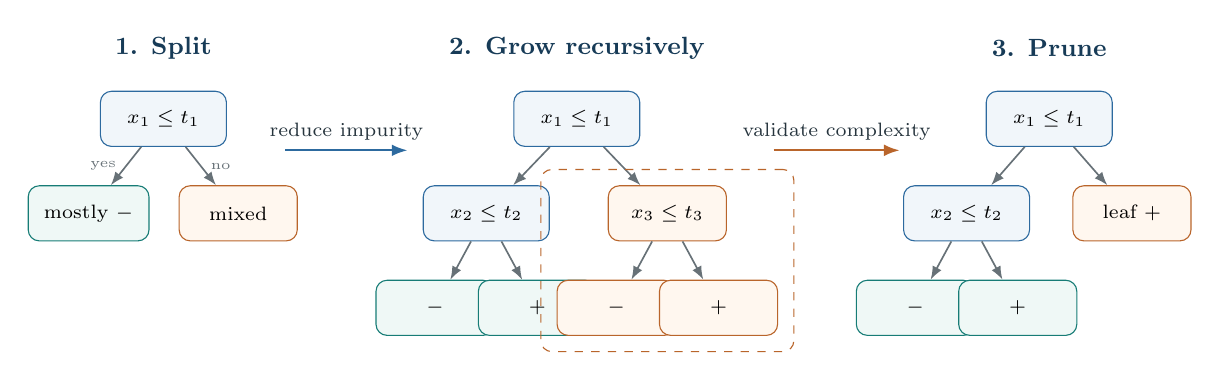
\begin{tikzpicture}[
  split/.style={draw=Blue,rounded corners,fill=PaleBlue,align=center,
    minimum width=16mm,minimum height=7mm,inner xsep=2mm,font=\scriptsize},
  leaf/.style={draw=Teal,rounded corners,fill=PaleTeal,align=center,
    minimum width=15mm,minimum height=7mm,inner xsep=2mm,font=\scriptsize},
  weak/.style={draw=Orange,rounded corners,fill=PaleOrange,align=center,
    minimum width=15mm,minimum height=7mm,inner xsep=2mm,font=\scriptsize},
  edge/.style={-{Latex[length=1.7mm]},semithick,color=Ink!70},
  stage/.style={font=\small\bfseries,color=Navy}
]
% Stage 1: one greedy split.
\node[stage] at (0,2.55) {1. Split};
\node[split] (a0) at (0,1.65) {$x_1\le t_1$};
\node[leaf] (a1) at (-0.95,0.45) {mostly $-$};
\node[weak] (a2) at (0.95,0.45) {mixed};
\draw[edge] (a0)--node[left,font=\tiny]{yes}(a1);
\draw[edge] (a0)--node[right,font=\tiny]{no}(a2);

% Stage 2: recursively split eligible non-pure children.
\node[stage] at (5.25,2.55) {2. Grow recursively};
\node[split] (b0) at (5.25,1.65) {$x_1\le t_1$};
\node[split] (b1) at (4.10,0.45) {$x_2\le t_2$};
\node[weak] (b2) at (6.40,0.45) {$x_3\le t_3$};
\node[leaf] (b11) at (3.45,-0.75) {$-$};
\node[leaf] (b12) at (4.75,-0.75) {$+$};
\node[weak] (b21) at (5.75,-0.75) {$-$};
\node[weak] (b22) at (7.05,-0.75) {$+$};
\draw[edge] (b0)--(b1); \draw[edge] (b0)--(b2);
\draw[edge] (b1)--(b11); \draw[edge] (b1)--(b12);
\draw[edge] (b2)--(b21); \draw[edge] (b2)--(b22);
\node[draw=Orange,dashed,rounded corners,fit=(b2)(b21)(b22),
  inner sep=2mm] (weaksubtree) {};

% Stage 3: collapse a weak subtree after validation.
\node[stage] at (11.25,2.55) {3. Prune};
\node[split] (c0) at (11.25,1.65) {$x_1\le t_1$};
\node[split] (c1) at (10.20,0.45) {$x_2\le t_2$};
\node[weak] (c2) at (12.30,0.45) {leaf $+$};
\node[leaf] (c11) at (9.55,-0.75) {$-$};
\node[leaf] (c12) at (10.85,-0.75) {$+$};
\draw[edge] (c0)--(c1); \draw[edge] (c0)--(c2);
\draw[edge] (c1)--(c11); \draw[edge] (c1)--(c12);

\draw[-{Latex[length=2mm]},thick,Blue]
  (1.55,1.25)--node[above,font=\scriptsize,color=Ink]{reduce impurity}(3.10,1.25);
\draw[-{Latex[length=2mm]},thick,Orange]
  (7.75,1.25)--node[above,font=\scriptsize,color=Ink]{validate complexity}(9.35,1.25);
\end{tikzpicture}
\caption{A tree chooses a locally useful split, recursively splits eligible non-pure children while the pre-pruning conditions permit further growth, and may then prune a branch whose added complexity is not supported by validation data. Pruning replaces the highlighted subtree by one leaf.}
\label{fig:tree-growth-pruning}
\end{figure}}

\newcommand{\EnsembleWorkflowFigure}{%
\begin{figure}[htbp]
\centering
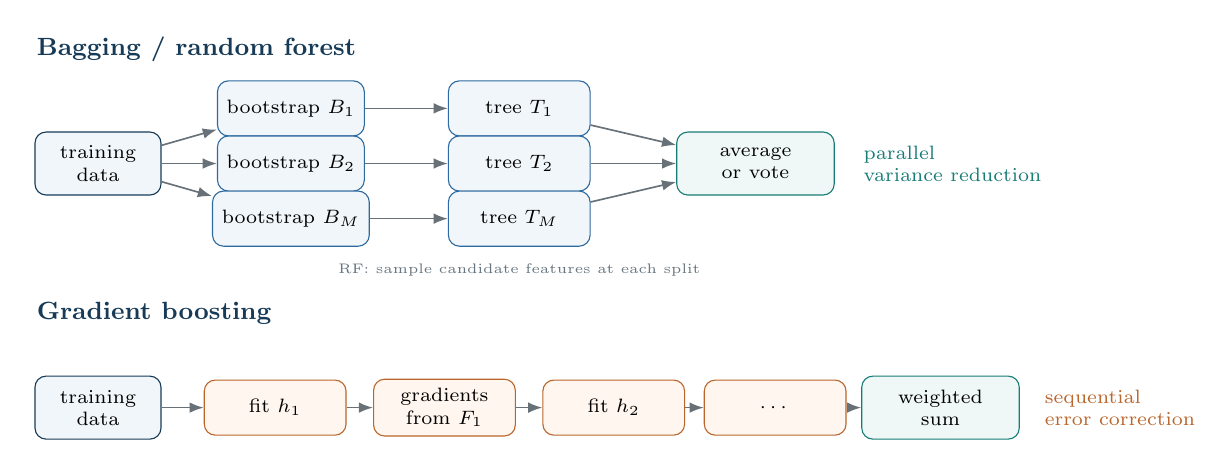
\begin{tikzpicture}[
  source/.style={draw=Navy,rounded corners,fill=PaleBlue,align=center,
    minimum width=16mm,minimum height=8mm,font=\scriptsize},
  bag/.style={draw=Blue,rounded corners,fill=PaleBlue,align=center,
    minimum width=18mm,minimum height=7mm,font=\scriptsize},
  boost/.style={draw=Orange,rounded corners,fill=PaleOrange,align=center,
    minimum width=18mm,minimum height=7mm,font=\scriptsize},
  output/.style={draw=Teal,rounded corners,fill=PaleTeal,align=center,
    minimum width=20mm,minimum height=8mm,font=\scriptsize},
  arr/.style={-{Latex[length=1.8mm]},semithick,color=Ink!70},
  lane/.style={font=\small\bfseries,color=Navy,anchor=west}
]
% Bagging and random-forest lane.
\node[lane] at (-0.15,3.00) {Bagging / random forest};
\node[source] (d1) at (0.75,1.55) {training\\data};
\node[bag] (s1) at (3.20,2.25) {bootstrap $B_1$};
\node[bag] (s2) at (3.20,1.55) {bootstrap $B_2$};
\node[bag] (sm) at (3.20,0.85) {bootstrap $B_M$};
\node[bag] (t1) at (6.10,2.25) {tree $T_1$};
\node[bag] (t2) at (6.10,1.55) {tree $T_2$};
\node[bag] (tm) at (6.10,0.85) {tree $T_M$};
\node[output] (agg) at (9.10,1.55) {average\\or vote};
\draw[arr] (d1)--(s1); \draw[arr] (d1)--(s2); \draw[arr] (d1)--(sm);
\draw[arr] (s1)--(t1); \draw[arr] (s2)--(t2); \draw[arr] (sm)--(tm);
\draw[arr] (t1)--(agg); \draw[arr] (t2)--(agg); \draw[arr] (tm)--(agg);
\node[font=\tiny,color=Muted] at (6.10,0.20)
  {RF: sample candidate features at each split};
\node[font=\scriptsize,color=Teal,anchor=west,align=left] at (10.35,1.55)
  {parallel\\variance reduction};

% Boosting lane.
\node[lane] at (-0.15,-0.35) {Gradient boosting};
\node[source] (d2) at (0.75,-1.55) {training\\data};
\node[boost] (h1) at (3.00,-1.55) {fit $h_1$};
\node[boost] (r2) at (5.15,-1.55) {gradients\\from $F_1$};
\node[boost] (h2) at (7.30,-1.55) {fit $h_2$};
\node[boost] (more) at (9.35,-1.55) {$\cdots$};
\node[output] (sum) at (11.45,-1.55) {weighted\\sum};
\draw[arr] (d2)--(h1); \draw[arr] (h1)--(r2); \draw[arr] (r2)--(h2);
\draw[arr] (h2)--(more); \draw[arr] (more)--(sum);
\node[font=\scriptsize,color=Orange,anchor=west,align=left] at (12.65,-1.55)
  {sequential\\error correction};
\end{tikzpicture}
\caption{Bagging fits learners independently on bootstrap samples and aggregates their predictions; a random forest additionally randomises candidate features at each split. Boosting is sequential: each learner follows the loss gradients of the current additive model.}
\label{fig:ensemble-workflows}
\end{figure}}


\section{Learning Problems and a Leakage-Free Workflow}
\label{sec:risk-workflow}

Supervised learning begins with labelled observations
\[
\mathcal D=\{(x_i,y_i)\}_{i=1}^{n},
\qquad x_i\in\mathbb R^d.
\]
The vector $x_i$ records the $d$ features of example $i$. In regression,
$y_i$ is usually real-valued. In classification, $y_i$ belongs to a finite set;
binary labels are commonly encoded as either $\{0,1\}$ or $\{-1,+1\}$.
Each encoding will be stated when it is used.

A model $f_\theta$ is determined by parameters $\theta$ and produces the
prediction $\hat y=f_\theta(x)$. A loss $\ell(y,\hat y)$ measures the error on
one example. Training usually minimises the empirical risk
\[
\widehat R(\theta)
=\frac{1}{n}\sum_{i=1}^{n}\ell\bigl(y_i,f_\theta(x_i)\bigr).
\]
The actual objective is low error on new examples from the same data-generating
distribution. If $(X,Y)$ denotes such an example, the relevant quantity is the
population risk
\[
R(\theta)=\mathbb E_{(X,Y)}
\left[\ell\bigl(Y,f_\theta(X)\bigr)\right].
\]
The population distribution is unknown, so $R(\theta)$ must be estimated using
data that did not determine the fitted model.

\subsection{Training, validation, and test sets}

A sound experiment splits the data before performing any operation that learns
from the data. The three subsets serve different purposes.
\begin{enumerate}
    \item The training set estimates model parameters, such as linear weights,
    tree split points, or neural-network weights.
    \item The validation set selects model classes and hyperparameters, such as
    the number of neighbours, tree depth, or the SVM penalty $C$.
    \item The test set is used once, after all choices have been fixed, to
    estimate the generalisation error of the final procedure.
\end{enumerate}

The word \emph{model} includes the complete preprocessing pipeline. Imputation,
standardisation, feature selection, dimensionality reduction, and resampling
may all learn properties of a dataset. They must therefore be fitted using only
the training data. For example, standardisation uses
\[
z_{ij}=\frac{x_{ij}-\mu_j}{s_j},
\]
where $\mu_j$ and $s_j$ are estimated from the training set. The same values
are then applied to validation and test examples. Estimating them from the full
dataset allows information from the test set to enter training and produces an
optimistic test error.

After hyperparameters have been selected, the final model may be refitted on
the union of the training and validation sets. Every preprocessing parameter
must then be re-estimated on that union, while the test set remains untouched.
Using test results to revise the model turns the test set into another
validation set and invalidates its role as an independent evaluation.

\subsection{The experimental data flow}

For a fixed family of candidate procedures, the data flow is
\[
\mathcal D_{\mathrm{train}}
\xrightarrow{\text{fit preprocessing and model}}
f_{\theta}
\xrightarrow{\mathcal D_{\mathrm{val}}}
\text{select hyperparameters}
\xrightarrow{\text{refit}}
f_{\mathrm{final}}
\xrightarrow{\mathcal D_{\mathrm{test}}}
\text{report error}.
\]
When the dataset is small, cross-validation within the training data can
replace a single validation split. Preprocessing must be refitted inside every
fold using only that fold's training portion.

\TrainingPipelineFigure


\section{Distance, Scaling, and Nearest Neighbours}

K-nearest neighbours (KNN) assumes that nearby observations tend to have
similar labels. Whether this assumption is useful depends first on the feature
representation and distance function. Different distances encode different
notions of similarity and are not interchangeable.

\subsection{Distances and similarities}

For $x,z\in\mathbb R^d$, the Euclidean and Manhattan distances are
\[
d_2(x,z)=\left(\sum_{j=1}^{d}(x_j-z_j)^2\right)^{1/2},
\qquad
d_1(x,z)=\sum_{j=1}^{d}|x_j-z_j|.
\]
Euclidean distance is the straight-line distance and gives relatively large
weight to a large discrepancy in one coordinate. Manhattan distance adds
absolute coordinate-wise discrepancies and is less dominated by such a
discrepancy.

When direction matters more than magnitude, cosine similarity is often more
appropriate for non-zero vectors $x$ and $z$:
\[
\operatorname{cos}(x,z)=\frac{x^\top z}
{\lVert x\rVert_2\lVert z\rVert_2}.
\]
The associated cosine distance is
$d_{\cos}(x,z)=1-\operatorname{cos}(x,z)$. Cosine similarity is not Euclidean
distance. After both vectors have been normalised to unit length, however,
\[
\left\lVert\frac{x}{\lVert x\rVert_2}-
\frac{z}{\lVert z\rVert_2}\right\rVert_2^2
=2\bigl(1-\operatorname{cos}(x,z)\bigr).
\]

For sets or binary features, Jaccard similarity ignores features that are absent
from both observations. If $A$ and $B$ are the sets of non-zero features, then
\[
J(A,B)=\frac{|A\cap B|}{|A\cup B|},
\qquad
d_J(A,B)=1-J(A,B).
\]
This definition is well suited to sparse presence--absence data because a
shared zero does not increase similarity. If $A=B=\varnothing$, the displayed
ratio is undefined; applications that permit empty sets must state a convention,
commonly $J(\varnothing,\varnothing)=1$.

\subsection{Feature scaling}

Distances are sensitive to units. If one feature is measured in thousands and
another lies between $0$ and $1$, the first feature can dominate every
Euclidean distance. Two common transformations are standardisation
\[
z_{ij}=\frac{x_{ij}-\mu_j}{s_j}
\]
and min--max scaling
\[
z_{ij}=\frac{x_{ij}-a_j}{b_j-a_j},
\]
where $a_j$ and $b_j$ are the minimum and maximum of feature $j$ in the
training set. Standardisation does not confine values to a fixed interval, but
it is usually less dependent on two observed endpoints. In either case, all
statistics are estimated from the training data alone. A constant feature has
$s_j=0$ and $b_j-a_j=0$; remove it or map it to a fixed value rather than divide
by zero.

Scaling is not an automatic requirement. Binary indicators, variables with a
meaningful physical scale, and inputs to decision trees need not receive the
same treatment. The choice follows from how the model uses each feature.

\subsection{The curse of dimensionality}
\label{sec:knn-dimensionality}

With a fixed number of observations, the sample becomes sparse as the dimension
increases. In a unit hypercube, a smaller hypercube of side length $r$ occupies
the fraction $r^d$ of the total volume. To enclose a fixed fraction $q$ of the
volume, its side length must be
\[
r=q^{1/d}.
\]
As $d$ increases, $r$ approaches $1$. A neighbourhood must therefore extend
through much of every coordinate range before it contains a fixed fraction of
the observations; it is no longer genuinely local.

Many high-dimensional distributions also exhibit distance concentration: the
relative difference between the nearest and farthest distances shrinks. The
distances remain computable, but their ranking carries less information. For
KNN, high dimensionality primarily causes sparse neighbourhoods and distance
concentration, which can in turn increase variance. More observations, feature
selection, dimensionality reduction, or a structured similarity measure may be
needed.

\subsection{K-nearest neighbours}

For a query $x$, KNN finds the $k$ training observations with the smallest
distance and denotes their index set by $N_k(x)$. A classifier uses a majority
vote,
\[
\hat y
=\operatorname*{arg\,max}_{c}
\sum_{i\in N_k(x)}\mathbf 1(y_i=c),
\]
whereas a regressor commonly uses the mean
\[
\hat y=\frac{1}{k}\sum_{i\in N_k(x)}y_i.
\]
Closer observations can be given more weight. One possible choice is
\[
w_i(x)=\frac{1}{d(x,x_i)+\varepsilon},
\qquad
\hat y
=\frac{\sum_{i\in N_k(x)}w_i(x)y_i}
{\sum_{i\in N_k(x)}w_i(x)}.
\]
where $\varepsilon>0$. The same weights can be used for a weighted class vote.

\KnnGeometryFigure

The value of $k$ controls smoothness. A small $k$ preserves local structure but
is sensitive to noise and individual outliers. A large $k$ is more stable but
may erase a genuine boundary. The rule $k=\sqrt n$ is at most an initial
heuristic; validation or cross-validation must determine the final value. An
odd $k$ reduces ties in binary classification, although ties can still occur
with several classes or repeated distances and therefore require an explicit
tie-breaking rule.

KNN has little explicit training cost but stores the training set. A brute-force
implementation computes $n$ distances in $d$ dimensions for each query, giving
time $O(nd)$ and storage $O(nd)$. Tree-based indices can accelerate low-dimensional
queries, but their benefit often declines in high dimensions.


\section{Decision Trees and Ensembles}

A decision tree partitions the input space recursively. Each internal node asks
a question about a feature, and each leaf stores a prediction. For a continuous
feature, a common split is
\[
x_j\le t,
\]
where $j$ selects a feature and $t$ is a threshold. For the observations $S$ at
the current node, the split produces
\[
S_L=\{(x_i,y_i)\in S:x_{ij}\le t\},
\qquad
S_R=S\setminus S_L.
\]
The two subsets need not have equal size. Training selects the split that most
reduces label impurity or numerical dispersion and repeats the process at the
child nodes.

\subsection{Impurity in classification trees}

Let $p_c$ be the proportion of class $c$ at node $S$. Entropy and Gini
impurity are
\[
H(S)=-\sum_{c=1}^{C}p_c\log_2 p_c,
\qquad
G(S)=1-\sum_{c=1}^{C}p_c^2,
\]
with the convention $0\log 0=0$. Both are zero at a pure node and increase as
the class distribution becomes more mixed.

Suppose a split produces child nodes of sizes $n_L$ and $n_R$, where
$n_S=n_L+n_R$. For an impurity measure $I$, the reduction is
\[
\Delta I
=I(S)-\frac{n_L}{n_S}I(S_L)
-\frac{n_R}{n_S}I(S_R).
\]
When $I=H$, this reduction is the information gain. A greedy tree normally
chooses the feature and threshold with the largest $\Delta I$.

For example, a node containing six positive and four negative examples has
entropy
\[
H(S)=-0.6\log_2 0.6-0.4\log_2 0.4\approx0.971.
\]
Suppose a split sends four positive examples to the left and the remaining two
positive and four negative examples to the right. The weighted child entropy is
\[
\frac{4}{10}\cdot0+
\frac{6}{10}\left(-\frac13\log_2\frac13-
\frac23\log_2\frac23\right)
\approx0.551,
\]
so the information gain is approximately $0.420$. The weighting accounts for
both child purity and child size; inspecting only one child is insufficient.

A classification leaf can output its majority class or estimated class
proportions,
\[
\widehat P(Y=c\mid x)=\frac{n_c}{n_{\mathrm{leaf}}}.
\]
The latter permits threshold adjustment, although probabilities estimated from
small leaves are unstable.

\subsection{Regression trees}

A regression tree uses the same partitioning mechanism. A leaf predicts its
mean response
\[
\bar y_S=\frac{1}{|S|}\sum_{i\in S}y_i.
\]
A common node impurity is the within-node sum of squared errors
\[
I_{\mathrm{reg}}(S)=
\sum_{i\in S}(y_i-\bar y_S)^2.
\]
Training selects the split that maximises
\[
I_{\mathrm{reg}}(S)
-I_{\mathrm{reg}}(S_L)
-I_{\mathrm{reg}}(S_R).
\]
The fitted function is constant within each leaf region, so a single regression
tree produces a piecewise-constant predictor.

\subsection{Stopping and pruning}

If a tree is allowed to keep splitting, a leaf may contain only one observation.
The resulting tree has low training error and high variance. Pre-pruning limits
growth directly through a maximum depth, a minimum leaf size, or a minimum
impurity reduction. Post-pruning first grows a larger tree and then removes
branches whose improvement is not supported by validation data.

\DecisionTreeLifecycleFigure

Cost-complexity pruning penalises the number of leaves:
\[
R_\alpha(T)=R(T)+\alpha |\mathcal L(T)|,
\]
where $R(T)$ is the training loss of tree $T$, $\mathcal L(T)$ is its set of
leaves, and $\alpha\ge0$. Larger values of $\alpha$ favour smaller trees. The
penalty is selected using validation data.

A prediction visits only the path from the root to a leaf, so its cost is
$O(h)$ for tree depth $h$. A balanced tree can have logarithmic depth, whereas
a degenerate tree can have depth linear in its number of leaves. Training cost
depends on how candidate thresholds are generated and sorted; it cannot be
described by a universal $O(dn^2\log n)$ expression.

\subsection{Bagging and random forests}

A deep tree can fit a complicated boundary, but small changes in the training
sample may alter its upper splits. Bagging constructs $M$ bootstrap samples.
Each contains $n$ observations drawn with replacement from the original sample.
The base learners are fitted separately, then averaged in regression or combined
by majority vote or mean class probability in classification:
\[
\bar f(x)=\frac1M\sum_{m=1}^{M}f_m(x).
\]

Suppose the prediction of each base learner at a fixed $x$ has variance
$\sigma^2$, and any pair has approximately the same correlation $\rho$. Then
\begin{equation}
\operatorname{Var}[\bar f(x)]
=\sigma^2\left(\rho+\frac{1-\rho}{M}\right).
\label{eq:correlated-ensemble-variance}
\end{equation}
The variance becomes $\sigma^2/M$ only when the predictors are independent
($\rho=0$). Trees trained on related bootstrap samples remain correlated, so
the reduction is smaller and depends on how effectively the procedure
decorrelates them.

A random forest adds feature randomisation. At each node, the tree searches for
a split among only $m_{\mathrm{try}}$ randomly selected features. This prevents
every tree from repeatedly relying on the same strong feature. The setting
$m_{\mathrm{try}}\approx\sqrt d$ is a common classification default, not a
theoretical optimum; regression implementations often use a different default.
The feature count, tree depth, and leaf size remain hyperparameters.

\EnsembleWorkflowFigure

\subsection{Boosting and gradient boosting}

Bagged learners can be trained in parallel. Boosting adds learners sequentially,
so that each new learner addresses errors of the current ensemble. An additive
model has the form
\[
F_M(x)=F_0(x)+\sum_{m=1}^{M}\eta\,\gamma_m h_m(x),
\]
where $h_m$ is often a shallow tree and $\eta\in(0,1]$ is the learning rate.

Gradient boosting applies this construction to a differentiable loss
$\ell(y,F(x))$. At iteration $m$, it computes the negative gradient at each
training observation,
\[
r_i^{(m)}=-\left.
\frac{\partial\ell(y_i,F(x_i))}{\partial F(x_i)}
\right|_{F=F_{m-1}},
\]
and fits $h_m$ to $\{(x_i,r_i^{(m)})\}$. A line search may choose
\[
\gamma_m=
\operatorname*{arg\,min}_{\gamma}
\sum_{i=1}^{n}
\ell\bigl(y_i,F_{m-1}(x_i)+\gamma h_m(x_i)\bigr),
\]
followed by
\[
F_m(x)=F_{m-1}(x)+\eta\gamma_mh_m(x).
\]
For squared loss $\ell(y,F)=\tfrac12(y-F)^2$, the negative gradient is the
residual $y_i-F_{m-1}(x_i)$. Fitting residuals is therefore the squared-loss
instance of gradient boosting, not its definition for every loss.

Boosting typically reduces bias, while tree depth, learning rate, and the number
of rounds determine capacity and variance. Select the number of rounds by
validation or early stopping.


\section{Regression and Classification from a Linear Score}

Several linear models share the score
\[
s(x)=w^\top x+b.
\]
They differ in how they interpret the score, which loss they minimise, and
whether they impose a margin. Linear regression uses $s(x)$ as a numerical
prediction. Logistic regression maps it to a probability. The Perceptron and
SVM classify according to its sign.

\subsection{Linear regression and the normal equations}
\label{sec:linear-score-regression}

Linear regression takes the score itself as the prediction,
$\hat y_i=s(x_i)$. With the intercept absorbed into an augmented design matrix
$X$ and parameter vector $\theta$, its squared-error objective is
\[
L(\theta)=\frac{1}{2n}\lVert X\theta-y\rVert_2^2.
\]
The derivation of the normal equations, the rank condition for the inverse
formula, and the regularised solution are given in
Section~\ref{sec:least-squares}. Linear regression uses the score directly;
unlike the classifiers below, it neither thresholds the score nor maps it to a
probability.

\subsection{Logistic regression}

Let $y_i\in\{0,1\}$. Logistic regression maps the linear score to a probability:
\[
p_i=P(Y=1\mid x_i)=\sigma(s_i),
\qquad
s_i=w^\top x_i+b,
\qquad
\sigma(z)=\frac{1}{1+e^{-z}}.
\]
Consequently,
\[
P(Y=y_i\mid x_i)=p_i^{y_i}(1-p_i)^{1-y_i}.
\]
Under conditional independence of the observations, maximum conditional
likelihood is equivalent to minimising the mean negative log-likelihood
\begin{align*}
L(w,b)
&=-\frac1n\sum_{i=1}^{n}
\left[y_i\log p_i+(1-y_i)\log(1-p_i)\right]\\
&=\frac1n\sum_{i=1}^{n}
\left[\log(1+e^{s_i})-y_is_i\right].
\end{align*}
This is binary cross-entropy. With the augmented design matrix $X$ and
$p=(p_1,\ldots,p_n)^\top$, its gradient is
\[
\nabla_\theta L=\frac1nX^\top(p-y).
\]
The optimisation procedure is developed in Section~\ref{sec:least-squares} and
the gradient-descent section that follows it.

The threshold $p_i\ge0.5$ is equivalent to $s_i\ge0$, so the decision boundary
is $w^\top x+b=0$. Changing the probability threshold changes the classifier
without refitting the probability model. With labels $y_i\in\{-1,+1\}$, the
same loss is
\[
\ell_{\mathrm{log}}(y_i,s_i)
=\log\bigl(1+e^{-y_is_i}\bigr).
\]

\subsection{The Perceptron}
\label{sec:perceptron}

The Perceptron uses labels $y_i\in\{-1,+1\}$ and predicts
\[
\widehat y_i=\operatorname{sign}(w^\top x_i+b).
\]
An observation is correctly classified when $y_is_i>0$. On a misclassified
observation, the update is
\[
w\leftarrow w+\eta y_ix_i,
\qquad
b\leftarrow b+\eta y_i.
\]
This update is a subgradient step on the Perceptron loss
\[
\ell_{\mathrm{perc}}(y_i,s_i)=\max(0,-y_is_i).
\]
The loss becomes zero as soon as the sign is correct and does not reward a wider
margin. For linearly separable training data, the Perceptron reaches a separating
hyperplane after finitely many updates. It need not find the maximum-margin
hyperplane and does not directly produce class probabilities. On non-separable
data, the original algorithm may continue updating without convergence.

\subsection{Maximum margin and hard-margin SVM}

Many separating hyperplanes may exist for linearly separable data. SVM fixes a
functional-margin scale and selects the hyperplane with the largest geometric
margin. The hard-margin primal problem is
\begin{align*}
\min_{w,b}\quad &\frac12\lVert w\rVert_2^2\\
\text{s.t.}\quad &y_i(w^\top x_i+b)\ge1,
\qquad i=1,\ldots,n.
\end{align*}
The signed distance from $x_i$ to $w^\top x+b=0$ is
$(w^\top x_i+b)/\lVert w\rVert_2$. Under the constraints, the closest training
points lie on $w^\top x+b=\pm1$, and the distance between these support
hyperplanes is
\[
\frac{2}{\lVert w\rVert_2}.
\]
Minimising $\tfrac12\lVert w\rVert_2^2$ therefore maximises the margin. The
hard-margin problem is feasible only when the training data are linearly
separable.

\LinearMarginFigure

\subsection{Soft-margin SVM and hinge loss}

Slack variables $\xi_i\ge0$ allow margin violations, with $C>0$ controlling
their penalty:
\begin{align*}
\min_{w,b,\xi}\quad
&\frac12\lVert w\rVert_2^2+C\sum_{i=1}^{n}\xi_i\\
\text{s.t.}\quad
&y_i(w^\top x_i+b)\ge1-\xi_i,
\qquad \xi_i\ge0.
\end{align*}
For fixed $w,b$, the optimal slack is
\[
\xi_i=\max\bigl(0,1-y_i(w^\top x_i+b)\bigr).
\]
The primal problem is therefore equivalent to
\[
\min_{w,b}\quad
\frac12\lVert w\rVert_2^2
+C\sum_{i=1}^{n}
\underbrace{\max(0,1-y_is_i)}_{\text{hinge loss}}.
\]
A large $C$ penalises violations heavily and favours fitting more training
observations. A small $C$ permits more violations in exchange for a wider
margin. Another common convention writes the objective as
$\lambda\lVert w\rVert_2^2/2+(1/n)\sum_i\ell_i$. The two conventions correspond
under a change of scale; values of $C$ and $\lambda$ cannot be compared without
specifying the objective.

Logistic regression, the Perceptron, and SVM all depend on the signed margin
$ys$, but use different losses:
\[
\begin{aligned}
\ell_{\mathrm{log}}(y,s)&=\log(1+e^{-ys}),\\
\ell_{\mathrm{perc}}(y,s)&=\max(0,-ys),\\
\ell_{\mathrm{hinge}}(y,s)&=\max(0,1-ys).
\end{aligned}
\]
Logistic loss is smooth and admits a probability interpretation. Perceptron
loss vanishes once the sign is correct. Hinge loss requires a functional margin
of at least $1$.

\subsection{The SVM dual}

The dual form of soft-margin SVM depends on the inputs only through inner
products. Introduce multipliers $\alpha_i\ge0$ for the margin constraints and
$\mu_i\ge0$ for $\xi_i\ge0$. The Lagrangian is
\begin{align*}
\mathcal L(w,b,\xi,\alpha,\mu)
=&\ \frac12\lVert w\rVert_2^2+C\sum_i\xi_i\\
&-\sum_i\alpha_i
\left[y_i(w^\top x_i+b)-1+\xi_i\right]
-\sum_i\mu_i\xi_i.
\end{align*}
Stationarity with respect to the primal variables gives
\[
\frac{\partial\mathcal L}{\partial w}=0
\ \Longrightarrow
w=\sum_i\alpha_i y_ix_i,
\]
\[
\frac{\partial\mathcal L}{\partial b}=0
\ \Longrightarrow
\sum_i\alpha_i y_i=0,
\qquad
\frac{\partial\mathcal L}{\partial\xi_i}=0
\ \Longrightarrow
C-\alpha_i-\mu_i=0.
\]
Since $\mu_i\ge0$, the last relation yields $0\le\alpha_i\le C$. Substitution
into the Lagrangian gives the dual problem
\begin{align*}
\max_{\alpha}\quad
&\sum_{i=1}^{n}\alpha_i
-\frac12\sum_{i=1}^{n}\sum_{j=1}^{n}
\alpha_i\alpha_jy_iy_jx_i^\top x_j\\
\text{s.t.}\quad
&0\le\alpha_i\le C,
\qquad
\sum_{i=1}^{n}\alpha_i y_i=0.
\end{align*}
The hard-margin dual has the same objective and equality constraint, but only
$\alpha_i\ge0$ and no upper bound $C$.

Observations with $\alpha_i>0$ appear in
$w=\sum_i\alpha_i y_ix_i$ and are the support vectors. If
$0<\alpha_i<C$, complementary slackness gives
\[
y_i(w^\top x_i+b)=1.
\]
Hence any such support vector gives
\[
b=y_i-\sum_j\alpha_jy_jx_j^\top x_i.
\]
Numerical implementations commonly average this value over several support
vectors satisfying $0<\alpha_i<C$.

\subsection{Kernel SVM}

Both the dual objective and the prediction function require only inner
products. If a feature map $\phi$ exists, a kernel
\[
K(x,z)=\phi(x)^\top\phi(z)
\]
can replace the original inner product without explicitly constructing the
possibly high-dimensional vector $\phi(x)$. The dual becomes
\begin{align*}
\max_{\alpha}\quad
&\sum_i\alpha_i
-\frac12\sum_i\sum_j
\alpha_i\alpha_jy_iy_jK(x_i,x_j)\\
\text{s.t.}\quad
&0\le\alpha_i\le C,
\qquad \sum_i\alpha_i y_i=0,
\end{align*}
and the prediction is
\[
\widehat y(x)=\operatorname{sign}
\left(\sum_{i=1}^{n}\alpha_i y_iK(x_i,x)+b\right).
\]
Only support vectors with $\alpha_i>0$ contribute to this sum.

Common kernels include the linear kernel
\[
K_{\mathrm{linear}}(x,z)=x^\top z,
\]
the polynomial kernel
\[
K_{\mathrm{poly}}(x,z)=(\gamma x^\top z+r)^q,
\qquad \gamma>0,\quad r\ge0,\quad q\in\{1,2,\ldots\},
\]
and the radial basis function kernel
\[
K_{\mathrm{RBF}}(x,z)=
\exp\bigl(-\gamma\lVert x-z\rVert_2^2\bigr),
\qquad \gamma>0.
\]
For a valid kernel, the Gram matrix $K_{ij}=K(x_i,x_j)$ must be positive
semidefinite for every finite set of inputs. In the RBF kernel, a larger $\gamma$ gives each observation a
narrower region of influence and usually permits a more intricate boundary; a
smaller $\gamma$ gives a smoother boundary. The values of $C$ and $\gamma$
jointly control model capacity and should be selected by the leakage-free
validation procedure described earlier.

% Additional vector figures for optimisation, regularisation, and evaluation.

\newcommand{\OptimisationPathFigure}{%
\begin{figure}[htbp]
\centering
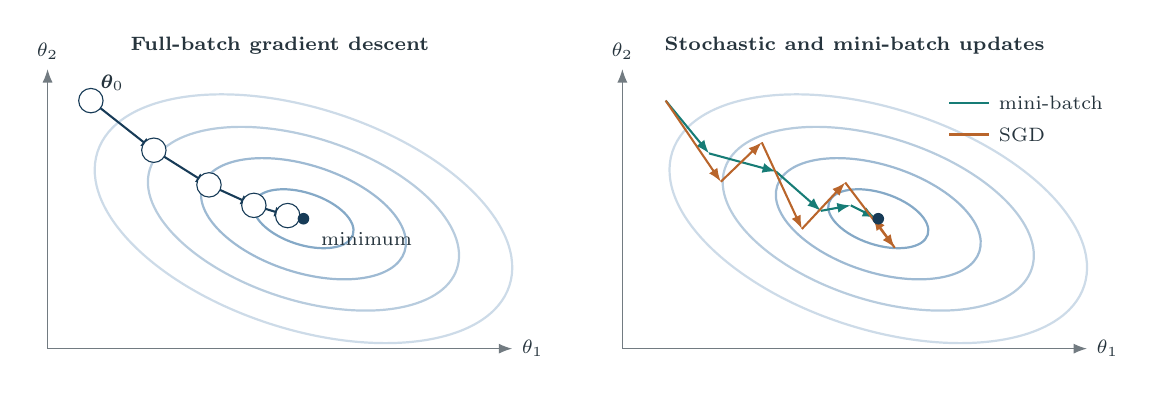
\begin{tikzpicture}[
  point/.style={circle,fill=white,draw,minimum size=3.1mm,inner sep=0pt},
  pathstep/.style={-{Latex[length=1.7mm]},line width=0.75pt},
  axis/.style={-{Latex[length=1.7mm]},color=Ink!65},
  label/.style={font=\scriptsize,color=Ink}
]
\node[label,font=\scriptsize\bfseries] at (3.15,4.05) {Full-batch gradient descent};
\node[label,font=\scriptsize\bfseries] at (10.45,4.05) {Stochastic and mini-batch updates};

\begin{scope}
  \draw[axis] (0.2,0.2)--(6.1,0.2) node[right,label] {$\theta_1$};
  \draw[axis] (0.2,0.2)--(0.2,3.75) node[above,label] {$\theta_2$};
  \begin{scope}[shift={(3.45,1.85)},rotate=-18]
    \draw[Blue!24,thick] (0,0) ellipse (2.75 and 1.40);
    \draw[Blue!34,thick] (0,0) ellipse (2.05 and 1.03);
    \draw[Blue!46,thick] (0,0) ellipse (1.35 and 0.68);
    \draw[Blue!58,thick] (0,0) ellipse (0.66 and 0.33);
  \end{scope}
  \coordinate (g0) at (0.75,3.35);
  \coordinate (g1) at (1.55,2.72);
  \coordinate (g2) at (2.25,2.28);
  \coordinate (g3) at (2.82,2.02);
  \coordinate (g4) at (3.25,1.89);
  \coordinate (g5) at (3.45,1.85);
  \foreach \a/\b in {g0/g1,g1/g2,g2/g3,g3/g4,g4/g5}
    \draw[pathstep,Navy] (\a)--(\b);
  \foreach \p in {g0,g1,g2,g3,g4}
    \node[point,draw=Navy] at (\p) {};
  \fill[Navy] (g5) circle (2.1pt);
  \node[label,anchor=south west] at (g0) {$\vect\theta_0$};
  \node[label,anchor=north west] at (3.55,1.80) {minimum};
\end{scope}

\begin{scope}[xshift=7.3cm]
  \draw[axis] (0.2,0.2)--(6.1,0.2) node[right,label] {$\theta_1$};
  \draw[axis] (0.2,0.2)--(0.2,3.75) node[above,label] {$\theta_2$};
  \begin{scope}[shift={(3.45,1.85)},rotate=-18]
    \draw[Blue!24,thick] (0,0) ellipse (2.75 and 1.40);
    \draw[Blue!34,thick] (0,0) ellipse (2.05 and 1.03);
    \draw[Blue!46,thick] (0,0) ellipse (1.35 and 0.68);
    \draw[Blue!58,thick] (0,0) ellipse (0.66 and 0.33);
  \end{scope}
  \coordinate (m0) at (0.75,3.35);
  \coordinate (m1) at (1.30,2.68);
  \coordinate (m2) at (2.15,2.45);
  \coordinate (m3) at (2.72,1.95);
  \coordinate (m4) at (3.10,2.02);
  \coordinate (m5) at (3.42,1.86);
  \foreach \a/\b in {m0/m1,m1/m2,m2/m3,m3/m4,m4/m5}
    \draw[pathstep,Teal] (\a)--(\b);
  \coordinate (s0) at (0.75,3.35);
  \coordinate (s1) at (1.45,2.32);
  \coordinate (s2) at (1.97,2.82);
  \coordinate (s3) at (2.48,1.72);
  \coordinate (s4) at (3.03,2.31);
  \coordinate (s5) at (3.66,1.48);
  \coordinate (s6) at (3.38,1.87);
  \foreach \a/\b in {s0/s1,s1/s2,s2/s3,s3/s4,s4/s5,s5/s6}
    \draw[pathstep,Orange] (\a)--(\b);
  \fill[Navy] (3.45,1.85) circle (2.1pt);
  \draw[Teal,line width=0.9pt] (4.35,3.32)--(4.85,3.32)
    node[right,label] {mini-batch};
  \draw[Orange,line width=0.9pt] (4.35,2.92)--(4.85,2.92)
    node[right,label] {SGD};
\end{scope}
\end{tikzpicture}
\caption{Optimisation paths on the same schematic loss contours. A full-batch gradient gives a deterministic direction for fixed parameters. Mini-batch and single-example gradients are random estimates of that direction; smaller batches usually produce larger step-to-step variation, even when the estimate is unbiased.}
\label{fig:optimisation-paths}
\end{figure}}

\newcommand{\RegularisationGeometryFigure}{%
\begin{figure}[htbp]
\centering
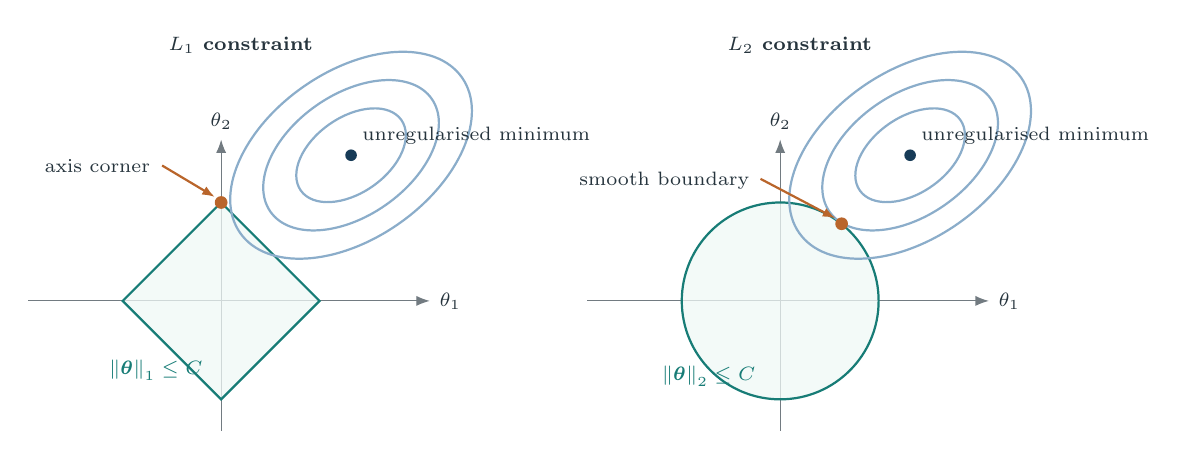
\begin{tikzpicture}[
  axis/.style={-{Latex[length=1.7mm]},color=Ink!65},
  contour/.style={Blue!55,thick},
  feasible/.style={Teal,thick,fill=PaleTeal,fill opacity=0.75},
  label/.style={font=\scriptsize,color=Ink}
]
\node[label,font=\scriptsize\bfseries] at (3.25,5.15) {$L_1$ constraint};
\node[label,font=\scriptsize\bfseries] at (10.35,5.15) {$L_2$ constraint};

\begin{scope}[shift={(3.0,1.9)}]
  \draw[axis] (-2.45,0)--(2.65,0) node[right,label] {$\theta_1$};
  \draw[axis] (0,-1.65)--(0,2.05) node[above,label] {$\theta_2$};
  \draw[feasible] (0,1.25)--(1.25,0)--(0,-1.25)--(-1.25,0)--cycle;
  \begin{scope}[shift={(1.65,1.85)},rotate=35]
    \draw[contour] (0,0) ellipse (0.78 and 0.48);
    \draw[contour] (0,0) ellipse (1.25 and 0.77);
    \draw[contour] (0,0) ellipse (1.72 and 1.06);
  \end{scope}
  \fill[Orange] (0,1.25) circle (2.3pt);
  \draw[Orange,-{Latex[length=1.6mm]},thick] (-0.75,1.72)--(-0.08,1.32);
  \node[label,anchor=e] at (-0.78,1.74) {axis corner};
  \fill[Navy] (1.65,1.85) circle (2.1pt);
  \node[label,anchor=south west] at (1.67,1.87) {unregularised minimum};
  \node[label,Teal] at (-0.83,-0.88) {$\norm{\vect\theta}_1\leq C$};
\end{scope}

\begin{scope}[shift={(10.1,1.9)}]
  \draw[axis] (-2.45,0)--(2.65,0) node[right,label] {$\theta_1$};
  \draw[axis] (0,-1.65)--(0,2.05) node[above,label] {$\theta_2$};
  \draw[feasible] (0,0) circle (1.25);
  \begin{scope}[shift={(1.65,1.85)},rotate=35]
    \draw[contour] (0,0) ellipse (0.78 and 0.48);
    \draw[contour] (0,0) ellipse (1.25 and 0.77);
    \draw[contour] (0,0) ellipse (1.72 and 1.06);
  \end{scope}
  \fill[Orange] (0.78,0.98) circle (2.3pt);
  \draw[Orange,-{Latex[length=1.6mm]},thick] (-0.25,1.55)--(0.70,1.05);
  \node[label,anchor=e] at (-0.27,1.57) {smooth boundary};
  \fill[Navy] (1.65,1.85) circle (2.1pt);
  \node[label,anchor=south west] at (1.67,1.87) {unregularised minimum};
  \node[label,Teal] at (-0.91,-0.96) {$\norm{\vect\theta}_2\leq C$};
\end{scope}
\end{tikzpicture}
\caption{Constrained views of regularisation. Expanding a loss contour from its unregularised minimum until it meets the feasible set gives the constrained solution. An $L_1$ ball has axis-aligned corners, so contact often sets a coefficient exactly to zero; the smooth $L_2$ boundary usually produces shrinkage without sparsity. The contact locations shown are schematic rather than universal.}
\label{fig:regularisation-geometry}
\end{figure}}

\newcommand{\ThresholdEvaluationFigure}{%
\begin{figure}[htbp]
\centering
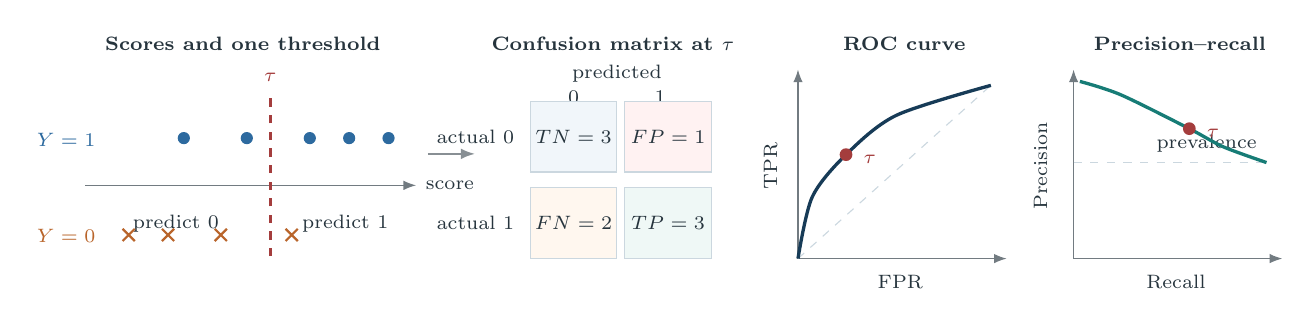
\begin{tikzpicture}[
  axis/.style={-{Latex[length=1.6mm]},color=Ink!65},
  flow/.style={-{Latex[length=1.8mm]},thick,color=Ink!55},
  label/.style={font=\scriptsize,color=Ink}
]
% Score and threshold.
\begin{scope}
  \node[label,font=\scriptsize\bfseries] at (2.0,3.45) {Scores and one threshold};
  \draw[axis] (0,1.65)--(4.2,1.65) node[right,label] {score};
  \draw[Red,dashed,thick] (2.35,0.75)--(2.35,2.85);
  \node[label,Red,above] at (2.35,2.85) {$\tau$};
  \node[label,anchor=north] at (1.15,1.40) {predict $0$};
  \node[label,anchor=north] at (3.30,1.40) {predict $1$};
  \foreach \x in {1.25,2.05,2.85,3.35,3.85}
    \fill[Blue] (\x,2.25) circle (2.2pt);
  \foreach \x in {0.55,1.05,1.72,2.62}
    \draw[Orange,thick] (\x,1.02) ++(-2.2pt,-2.2pt)--++(4.4pt,4.4pt)
      (\x,1.02) ++(-2.2pt,2.2pt)--++(4.4pt,-4.4pt);
  \node[label,Blue,anchor=e] at (0.25,2.25) {$Y=1$};
  \node[label,Orange,anchor=e] at (0.25,1.02) {$Y=0$};
\end{scope}

% Confusion matrix.
\begin{scope}[shift={(5.15,0.72)}]
  \node[label,font=\scriptsize\bfseries] at (1.55,2.73) {Confusion matrix at $\tau$};
  \node[label] at (1.60,2.35) {predicted};
  \node[label] at (1.05,2.05) {$0$};
  \node[label] at (2.15,2.05) {$1$};
  \node[label,anchor=east] at (0.42,1.55) {actual $0$};
  \node[label,anchor=east] at (0.42,0.45) {actual $1$};
  \fill[PaleBlue] (0.5,1.1) rectangle (1.6,2.0);
  \fill[PaleRed] (1.7,1.1) rectangle (2.8,2.0);
  \fill[PaleOrange] (0.5,0) rectangle (1.6,0.9);
  \fill[PaleTeal] (1.7,0) rectangle (2.8,0.9);
  \draw[Rule] (0.5,0) rectangle (1.6,0.9);
  \draw[Rule] (1.7,0) rectangle (2.8,0.9);
  \draw[Rule] (0.5,1.1) rectangle (1.6,2.0);
  \draw[Rule] (1.7,1.1) rectangle (2.8,2.0);
  \node[label] at (1.05,1.55) {$TN=3$};
  \node[label] at (2.25,1.55) {$FP=1$};
  \node[label] at (1.05,0.45) {$FN=2$};
  \node[label] at (2.25,0.45) {$TP=3$};
\end{scope}

% ROC panel.
\begin{scope}[shift={(9.05,0.72)}]
  \node[label,font=\scriptsize\bfseries] at (1.35,2.73) {ROC curve};
  \draw[axis] (0,0)--(2.65,0);
  \draw[axis] (0,0)--(0,2.40);
  \node[label] at (1.30,-0.30) {FPR};
  \node[label,rotate=90] at (-0.35,1.18) {TPR};
  \draw[Rule,dashed] (0,0)--(2.45,2.20);
  \draw[Navy,very thick] plot[smooth] coordinates
    {(0,0) (0.18,0.78) (0.61,1.32) (1.25,1.82) (2.45,2.20)};
  \fill[Red] (0.61,1.32) circle (2.3pt);
  \node[label,Red,anchor=west] at (0.71,1.26) {$\tau$};
\end{scope}

% Precision--recall panel.
\begin{scope}[shift={(12.55,0.72)}]
  \node[label,font=\scriptsize\bfseries] at (1.35,2.73) {Precision--recall};
  \draw[axis] (0,0)--(2.65,0);
  \draw[axis] (0,0)--(0,2.40);
  \node[label] at (1.30,-0.30) {Recall};
  \node[label,rotate=90] at (-0.42,1.18) {Precision};
  \draw[Rule,dashed] (0,1.22)--(2.45,1.22)
    node[above left,label] {prevalence};
  \draw[Teal,very thick] plot[smooth] coordinates
    {(0.08,2.25) (0.60,2.08) (1.47,1.65) (1.90,1.42) (2.45,1.22)};
  \fill[Red] (1.47,1.65) circle (2.3pt);
  \node[label,Red,anchor=west] at (1.57,1.59) {$\tau$};
\end{scope}

\draw[flow] (4.35,2.05)--(4.95,2.05);
\end{tikzpicture}
\caption{A threshold converts scores into predicted labels and therefore fixes one confusion matrix. That matrix gives one ROC point $(\mathrm{FPR},\mathrm{TPR})$ and one precision--recall point $(\mathrm{Recall},\mathrm{Precision})$. Sweeping the threshold traces both curves; the random-ranking baseline for Precision equals the positive-class prevalence.}
\label{fig:threshold-evaluation}
\end{figure}}


\section{Learning Model Parameters}

A model specifies a family of functions indexed by parameters $\vect\theta$.
Training selects one function from this family. Section~\ref{sec:risk-workflow}
defines population and empirical risk and explains why training fit alone does
not measure generalisation. Here the observations are assumed iid and drawn from
the deployment distribution unless stated otherwise; time dependence, grouping,
or distribution shift requires a different split and error analysis.

\subsection{Empirical Risk and Regularisation}

Regularised training adds a parameter preference to empirical risk:
\[
  J(\vect\theta)
  =\widehat R_n(\vect\theta)+\lambda\Omega(\vect\theta),
  \qquad \lambda\geq 0.
\]
The penalty $\Omega$ restricts effective model complexity, while $\lambda$ controls its strength relative to data fit.

\subsection{Least Squares and the Normal Equations}
\label{sec:least-squares}

For linear regression, let $X\in\R^{n\times d}$ have row $\vect x_i^{\top}$ and let $\vect y=(y_1,\ldots,y_n)^{\top}\in\R^n$. To include an intercept, define
\[
  \widetilde X=[\vect 1\;X]\in\R^{n\times(d+1)},
  \qquad
  \widetilde{\vect\theta}
  =\begin{bmatrix}b\\\vect w\end{bmatrix}\in\R^{d+1}.
\]
Then $f(\vect x)=b+\vect w^{\top}\vect x$, and the mean squared error is
\[
  L(\widetilde{\vect\theta})
  =\frac1n\norm{\widetilde X\widetilde{\vect\theta}-\vect y}_2^2.
\]
Expanding the quadratic gives
\begin{align*}
  L(\widetilde{\vect\theta})
  &=\frac1n(\widetilde X\widetilde{\vect\theta}-\vect y)^{\top}
    (\widetilde X\widetilde{\vect\theta}-\vect y)\\
  &=\frac1n\left(
      \widetilde{\vect\theta}^{\top}\widetilde X^{\top}\widetilde X
      \widetilde{\vect\theta}
      -2\widetilde{\vect\theta}^{\top}\widetilde X^{\top}\vect y
      +\vect y^{\top}\vect y
    \right),\\
  \nabla_{\widetilde{\vect\theta}}L(\widetilde{\vect\theta})
  &=\frac{2}{n}\widetilde X^{\top}
    (\widetilde X\widetilde{\vect\theta}-\vect y).
\end{align*}
Setting the gradient to zero yields the normal equations
\[
  \widetilde X^{\top}\widetilde X\widehat{\widetilde{\vect\theta}}
  =\widetilde X^{\top}\vect y.
\]
If $\widetilde X$ has full column rank, so that $\operatorname{rank}(\widetilde X)=d+1$, then $\widetilde X^{\top}\widetilde X$ is invertible and the unique solution is
\[
  \boxed{
  \widehat{\widetilde{\vect\theta}}
  =(\widetilde X^{\top}\widetilde X)^{-1}
    \widetilde X^{\top}\vect y.}
\]
If $\widetilde X$ is rank deficient, the least-squares solution need not be unique and this inverse must not be used. The minimum-norm solution is $\widetilde X^{+}\vect y$, where $\widetilde X^{+}$ is the Moore--Penrose pseudoinverse. Ridge regularisation provides another remedy by making the system matrix invertible.

\subsection{Gradient Descent, Mini-batches, and SGD}

Closed-form solutions are available for only a limited class of objectives. A differentiable objective $J(\vect\theta)$ can instead be minimised iteratively. Gradient descent evaluates the gradient at the current iterate:
\[
  \boxed{
  \vect\theta_{t+1}
  =\vect\theta_t-\eta_t\nabla J(\vect\theta_t),}
\]
where $\eta_t>0$ is the learning rate. The negative gradient is the direction of steepest local decrease under the Euclidean norm because
\[
  J(\vect\theta_t+\Delta\vect\theta)
  \approx J(\vect\theta_t)
  +\nabla J(\vect\theta_t)^{\top}\Delta\vect\theta.
\]
The gradient is evaluated at $\vect\theta_t$, not at the unknown $\vect\theta_{t+1}$. A learning rate that is too large can overshoot low-loss regions or cause divergence; a learning rate that is too small gives slow progress.

When the empirical objective decomposes as
$J(\vect\theta)=n^{-1}\sum_i\ell_i(\vect\theta)$, a full-batch update reads every observation. For a randomly sampled mini-batch $B_t\subseteq\{1,\ldots,n\}$, define
\[
  \vect g_t
  =\frac{1}{\abs{B_t}}
    \sum_{i\in B_t}\nabla\ell_i(\vect\theta_t),
  \qquad
  \vect\theta_{t+1}=\vect\theta_t-\eta_t\vect g_t.
\]
Under uniform sampling,
\[
  \E[\vect g_t\mid\vect\theta_t]=\nabla J(\vect\theta_t).
\]
The case $\abs{B_t}=1$ is stochastic gradient descent (SGD); values between $1$ and $n$ give mini-batch gradient descent. Small batches reduce the cost of an update but produce a noisier gradient estimate. Large batches give a more stable direction at a higher per-update cost. Stochastic updates can sometimes move away from flat saddle regions, but they do not guarantee a global optimum.

\OptimisationPathFigure

For an $L$-smooth convex objective, full-batch gradient descent converges in objective value under the fixed-step condition $0<\eta<2/L$. Convergence claims for SGD additionally require assumptions on sampling, gradient variance, and usually a decreasing step schedule. Neural-network objectives are generally non-convex; optimisation then seeks a low-loss stationary region, while validation measures generalisation.

\subsection{Maximum Likelihood Estimation}

A probabilistic model specifies a conditional distribution $p_{\vect\theta}(y\mid\vect x)$. Conditional independence of the labels gives the likelihood
\[
  p_{\vect\theta}(\vect y\mid X)
  =\prod_{i=1}^{n}p_{\vect\theta}(y_i\mid\vect x_i).
\]
Maximum likelihood estimation (MLE) is equivalent to minimising negative log-likelihood:
\begin{align*}
  \widehat{\vect\theta}_{\mathrm{MLE}}
  &\in\argmax_{\vect\theta}
    \prod_{i=1}^{n}p_{\vect\theta}(y_i\mid\vect x_i)\\
  &=\argmin_{\vect\theta}
    \left[-\sum_{i=1}^{n}\log p_{\vect\theta}(y_i\mid\vect x_i)\right].
\end{align*}
The logarithm turns a product into a sum and avoids numerical underflow from multiplying many small probabilities.

Squared error follows from a Gaussian noise model. Assume
\[
  y_i=f_{\vect\theta}(\vect x_i)+\varepsilon_i,
  \qquad
  \varepsilon_i\overset{\mathrm{iid}}{\sim}\mathcal N(0,\sigma^2),
\]
with a variance that does not depend on $\vect x_i$. Then
\[
  -\log p_{\vect\theta}(\vect y\mid X)
  =\frac n2\log(2\pi\sigma^2)
   +\frac{1}{2\sigma^2}
      \sum_{i=1}^{n}
      \bigl(y_i-f_{\vect\theta}(\vect x_i)\bigr)^2.
\]
For fixed $\sigma^2$, the first term is constant in $\vect\theta$, and the positive scale of the second term does not change its minimiser. MLE under independent homoscedastic Gaussian noise therefore gives the same estimate as least squares. If the conditional variance changes with the input, ordinary MSE is no longer the complete negative log-likelihood.

\subsection{MAP Estimation and Regularisation}

Maximum a posteriori estimation (MAP) places a prior distribution $p(\vect\theta)$ on the parameters:
\begin{align*}
  \widehat{\vect\theta}_{\mathrm{MAP}}
  &\in\argmax_{\vect\theta}p(\vect\theta\mid\mathcal D)\\
  &=\argmax_{\vect\theta}
    \left[\log p(\mathcal D\mid\vect\theta)+\log p(\vect\theta)\right].
\end{align*}
The evidence $p(\mathcal D)$ is independent of $\vect\theta$ and therefore does not affect the maximiser.

Suppose the parameter components are independent and follow zero-mean Gaussian priors:
\[
  \theta_j\sim\mathcal N(0,\tau^2),
  \qquad
  -\log p(\vect\theta)
  =\frac{1}{2\tau^2}\norm{\vect\theta}_2^2+\text{constant}.
\]
The resulting MAP objective has an $L_2$ penalty. Independent Laplace priors instead give
\[
  p(\theta_j)=\frac{1}{2b}
    \exp\!\left(-\frac{\abs{\theta_j}}{b}\right),
  \qquad
  -\log p(\vect\theta)
  =\frac1b\norm{\vect\theta}_1+\text{constant},
\]
which produces an $L_1$ penalty. The regularisation coefficient depends on both the likelihood scale and the prior scale. Replacing a summed loss by a mean loss also changes the corresponding numerical value of $\lambda$.

These correspondences require the stated independent, zero-centred priors. The intercept is commonly left unregularised because an overall shift should not be treated as a feature effect. MAP returns the posterior mode; it does not retain the uncertainty represented by the full posterior distribution.


\section{Generalisation, Regularisation, and Model Selection}

A training algorithm observes a finite sample but must predict on new inputs. Generalisation analysis treats the training set itself as random. Different samples produce different fitted functions, so test error contains systematic bias, sensitivity to the training sample, and noise in the data-generating process.

\subsection{Bias--Variance--Noise Decomposition}

Consider regression with squared loss. Define the regression function and conditional noise variance by
\[
  f^*(\vect x)=\E[Y\mid X=\vect x],
  \qquad
  \sigma^2(\vect x)=\Var(Y\mid X=\vect x).
\]
Equivalently,
\[
  Y=f^*(\vect x)+\varepsilon,
  \qquad
  \E[\varepsilon\mid\vect x]=0,
  \qquad
  \Var(\varepsilon\mid\vect x)=\sigma^2(\vect x).
\]
Let a random training set $\mathcal D$ produce the fitted function $\widehat f_{\mathcal D}$, and define its average prediction over possible training sets by
\[
  \overline f(\vect x)
  =\E_{\mathcal D}[\widehat f_{\mathcal D}(\vect x)].
\]
At a fixed input $\vect x$, the expected test error is
\begin{align*}
  &\E_{\mathcal D,Y\mid\vect x}
    \left[\bigl(\widehat f_{\mathcal D}(\vect x)-Y\bigr)^2\right]\\
  &=\E_{\mathcal D,Y\mid\vect x}
    \left[\bigl(
      \widehat f_{\mathcal D}(\vect x)-f^*(\vect x)-\varepsilon
    \bigr)^2\right]\\
  &=\E_{\mathcal D}
    \left[\bigl(
      \widehat f_{\mathcal D}(\vect x)-f^*(\vect x)
    \bigr)^2\right]
    +\sigma^2(\vect x).
\end{align*}
The cross term vanishes because $\E[\varepsilon\mid\vect x]=0$ and test-label noise is independent of the training set. Add and subtract $\overline f(\vect x)$ in the remaining expectation:
\begin{align*}
  &\E_{\mathcal D}
    \left[\bigl(
      \widehat f_{\mathcal D}(\vect x)-f^*(\vect x)
    \bigr)^2\right]\\
  &=\E_{\mathcal D}\left[
    \bigl(
      \widehat f_{\mathcal D}(\vect x)-\overline f(\vect x)
      +\overline f(\vect x)-f^*(\vect x)
    \bigr)^2\right]\\
  &=\underbrace{
      \E_{\mathcal D}\left[
        \bigl(
          \widehat f_{\mathcal D}(\vect x)-\overline f(\vect x)
        \bigr)^2
      \right]
    }_{\text{variance}}
    +\underbrace{
      \bigl(\overline f(\vect x)-f^*(\vect x)\bigr)^2
    }_{\text{squared bias}}.
\end{align*}
The second cross term is zero because
$\E_{\mathcal D}[\widehat f_{\mathcal D}(\vect x)-\overline f(\vect x)]=0$. Hence
\[
  \boxed{
  \E_{\mathcal D,Y\mid\vect x}
  \left[\bigl(\widehat f_{\mathcal D}(\vect x)-Y\bigr)^2\right]
  =\operatorname{Bias}^2(\vect x)
   +\Var_{\mathcal D}\!\left(\widehat f_{\mathcal D}(\vect x)\right)
   +\sigma^2(\vect x).}
\]
Taking an additional expectation over $X$ gives the decomposition of the overall test MSE. Bias measures the systematic difference between the average prediction and $f^*$. Variance measures sensitivity to the sampled training set. The term $\sigma^2(\vect x)$ is irreducible when predicting an individual response under squared loss. Bias is not irreducible noise. This exact identity is specific to squared loss; the same terms are used only qualitatively for most classification losses.

Increasing model flexibility often reduces bias and increases variance, but this is not a theorem that applies pointwise to every model family. The shape of the trade-off also depends on the optimiser, regularisation, and data distribution.

\BiasVarianceFigure

\subsection{\texorpdfstring{$L_1$ and $L_2$ Geometry}{L1 and L2 Geometry}}

Two common regularised objectives are
\[
  \min_{\vect\theta}
    \widehat R_n(\vect\theta)+\lambda\norm{\vect\theta}_2^2,
  \qquad
  \min_{\vect\theta}
    \widehat R_n(\vect\theta)+\lambda\norm{\vect\theta}_1.
\]
The $L_2$ penalty is smooth and encourages a smaller coefficient norm. In ridge regression, individual coordinates need not decrease monotonically when features are correlated. The penalty does not, by geometry alone, make many coefficients exactly zero. The $L_1$ ball has corners on the coordinate axes. A loss contour that first touches this boundary often does so at a corner, which produces a sparse solution. The $L_1$ norm is non-differentiable when a coordinate is zero, but it is convex and can be optimised with subgradients or coordinate descent.

\RegularisationGeometryFigure

The penalised and constrained forms are
\[
  \min_{\vect\theta}
    \widehat R_n(\vect\theta)+\lambda\Omega(\vect\theta),
  \qquad
  \min_{\vect\theta}\widehat R_n(\vect\theta)
  \quad\text{subject to}\quad
  \Omega(\vect\theta)\leq C.
\]
Under convexity, feasibility, and strong-duality conditions, a solution to the penalised problem corresponds to a constrained problem with
$C=\Omega(\widehat{\vect\theta})$. The mapping between $C$ and $\lambda$ need not be one-to-one, and the relation is not generally $C=1/\lambda$.

For ridge regression, use the augmented quantities above and define
$D=\diag(0,1,\ldots,1)$ so that the intercept is not penalised. The objective
\[
  J(\widetilde{\vect\theta})
  =\frac1n\norm{\widetilde X\widetilde{\vect\theta}-\vect y}_2^2
   +\lambda\widetilde{\vect\theta}^{\top}D\widetilde{\vect\theta}
\]
has gradient
\[
  \nabla J(\widetilde{\vect\theta})
  =\frac2n\widetilde X^{\top}
    (\widetilde X\widetilde{\vect\theta}-\vect y)
   +2\lambda D\widetilde{\vect\theta}.
\]
Setting it to zero gives
\[
  \boxed{
  \widehat{\widetilde{\vect\theta}}_{\mathrm{ridge}}
  =(\widetilde X^{\top}\widetilde X+n\lambda D)^{-1}
    \widetilde X^{\top}\vect y.}
\]
For $\lambda>0$ and $n>0$, $\widetilde X^{\top}\widetilde X+n\lambda D$ is positive definite and invertible: the data term identifies the intercept, while the penalty is positive on every non-zero slope vector.

\subsection{Holdout Validation}

Development data are commonly divided into a training set and a validation set, with a separate test set reserved for final evaluation. For each hyperparameter setting $h$, fit $\widehat f_h$ on the training set and compute
\[
  \widehat L_{\mathrm{val}}(h)
  =\frac1m\sum_{i=1}^{m}
    \ell\bigl(
      y_i^{\mathrm{val}},
      \widehat f_h(\vect x_i^{\mathrm{val}})
    \bigr).
\]
After selecting $h$, the model may be refitted on the combined training and validation data. The test set is then evaluated once; it must not be used for further tuning.

Suppose $h$ and the fitted model are fixed before validation, the validation observations are iid, and the per-example loss has conditional variance $\sigma_\ell^2$. Define the risk of this fixed fit as $R(\widehat f_h)$. Conditional on the training data,
\[
  \E[\widehat L_{\mathrm{val}}(h)\mid\mathcal D_{\mathrm{train}}]
  =R(\widehat f_h),
  \qquad
  \Var(\widehat L_{\mathrm{val}}(h)\mid\mathcal D_{\mathrm{train}})
  =\frac{\sigma_\ell^2}{m}.
\]
The standard error therefore decreases at rate $m^{-1/2}$. The notation $O(m^{-1/2})$ describes a scale of sampling fluctuation, not a deterministic identity of the form
$\widehat L_{\mathrm{val}}=L\pm O(m^{-1/2})$. If the same validation set selects among many hyperparameter settings, the smallest observed validation loss is subject to selection bias and cannot replace an independent test estimate.

\subsection{\texorpdfstring{$K$-Fold Cross-Validation}{K-Fold Cross-Validation}}

Partition the development data into disjoint folds $F_1,\ldots,F_K$. For fold $k$, fit $\widehat f_h^{(-k)}$ on the other $K-1$ folds and evaluate on $F_k$:
\[
  \widehat L_{\mathrm{CV}}(h)
  =\frac1K\sum_{k=1}^{K}
    \frac{1}{\abs{F_k}}
    \sum_{i\in F_k}
      \ell\bigl(y_i,\widehat f_h^{(-k)}(\vect x_i)\bigr).
\]
Each observation serves as validation data once. This procedure directly evaluates fits trained on approximately $\frac{K-1}{K}n$ observations, not the final model refitted on all development data.

Stratified folds preserve approximate class proportions in classification. Time-series observations must not be randomly shuffled; forward-chaining folds prevent future observations from predicting the past. If model selection and an approximately unbiased performance estimate are both required, nested cross-validation uses inner folds for selection and outer folds for evaluation.

\subsection{Early Stopping}

During iterative training, the training loss can continue to decrease after the validation loss begins to rise. If $\vect\theta_t$ denotes the parameters after update $t$, the stopping time can be selected by
\[
  t^*\in\argmin_t
    \widehat L_{\mathrm{val}}(\vect\theta_t),
  \qquad
  \widehat{\vect\theta}=\vect\theta_{t^*}.
\]
Training should restore the parameters from the best validation checkpoint rather than keep only the parameters at the final update. A patience window tolerates short fluctuations caused by mini-batch noise. Since the number of updates is selected through validation performance, early stopping is a form of model selection and implicit regularisation. The test set must not be monitored after every epoch.

\subsection{Correlation in Model Averaging}

Let $f_1,\ldots,f_K$ be base-model predictions at a fixed input, with average
\[
  \overline f_K=\frac1K\sum_{k=1}^{K}f_k.
\]
In general,
\[
  \Var(\overline f_K)
  =\frac{1}{K^2}
    \left(
      \sum_{k=1}^{K}\Var(f_k)
      +2\sum_{i<j}\Cov(f_i,f_j)
    \right).
\]
If every model has variance $\sigma_f^2$ and every pair has correlation $\rho$,
this reduces to Equation~\eqref{eq:correlated-ensemble-variance}. Variance falls
as $1/K$ only when $\rho=0$; for $\rho>0$, its limit is $\rho\sigma_f^2$.
Random forests randomise candidate features partly to reduce correlation among
trees. Averaging does not automatically reduce bias; bagging mainly reduces
variance for unstable learners.

\section{Model Evaluation and Class Imbalance}

An evaluation metric is meaningful only after the task, positive class, and decision costs have been specified. Define evaluation metrics before inspecting test results, and select decision thresholds on validation data.

\subsection{The Confusion Matrix and Basic Metrics}

For a positive class $Y=1$, the four counts are true positives $TP$, false positives $FP$, false negatives $FN$, and true negatives $TN$. They define
\begin{align*}
  \mathrm{Accuracy}
  &=\frac{TP+TN}{TP+TN+FP+FN},\\
  \mathrm{Precision}
  &=\frac{TP}{TP+FP},\\
  \mathrm{Recall}=\mathrm{TPR}
  &=\frac{TP}{TP+FN},\\
  \mathrm{Specificity}
  &=\frac{TN}{TN+FP},\\
  F_1
  &=\frac{2\,\mathrm{Precision}\cdot\mathrm{Recall}}
          {\mathrm{Precision}+\mathrm{Recall}}
    =\frac{2TP}{2TP+FP+FN}.
\end{align*}
Precision is the fraction of predicted positives that are correct. Recall is the fraction of positive examples that are correctly identified. The $F_1$ score is their harmonic mean and does not use $TN$. If a denominator is zero, software libraries may return zero, an undefined value, or a warning; a report should state the convention used.

\begin{examplebox}[Accuracy under class imbalance]
Consider a test set of $1000$ observations with only $60$ positives. If
$TP=40$, $FP=10$, $FN=20$, and $TN=930$, then
\[
  \mathrm{Accuracy}=0.97,
  \qquad
  \mathrm{Precision}=0.80,
  \qquad
  \mathrm{Recall}=\frac23,
  \qquad
  F_1\approx0.727.
\]
The $97\%$ accuracy conceals that the classifier misses one third of the positive examples.
\end{examplebox}

\subsection{Decision Thresholds and Costs}

Many classifiers first return a score $s(\vect x)$ or an estimated probability $\widehat p(Y=1\mid\vect x)$, then apply a threshold $\tau$:
\[
  \widehat y_\tau=\ind\{s(\vect x)\geq\tau\}.
\]
Lowering $\tau$ generally increases both $TP$ and $FP$. Recall therefore rises, while Precision may rise or fall. A threshold of $0.5$ is natural only under particular calibration and cost assumptions; it is not universally optimal.

If a false negative costs $C_{\mathrm{FN}}$ and a false positive costs $C_{\mathrm{FP}}$, choose the threshold on validation data by minimising
\[
  C(\tau)
  =C_{\mathrm{FN}}FN(\tau)+C_{\mathrm{FP}}FP(\tau).
\]
Ranking quality, probability calibration, and performance at a fixed threshold are distinct properties. AUC assesses ranking. Calibration curves or the Brier score assess probability calibration. Confusion-matrix metrics assess a particular decision rule.

\subsection{ROC, Precision--Recall, and AUC}

Varying $\tau$ gives
\[
  \mathrm{TPR}(\tau)
  =\frac{TP(\tau)}{TP(\tau)+FN(\tau)},
  \qquad
  \mathrm{FPR}(\tau)
  =\frac{FP(\tau)}{FP(\tau)+TN(\tau)}.
\]
The ROC curve plots TPR against FPR. AUROC is the area under this curve. For continuous scores, it is also the probability that a randomly selected positive receives a higher score than a randomly selected negative, with half credit for a tie. AUROC is unchanged by a strictly increasing transformation of the scores and does not assess probability calibration.

The precision--recall (PR) curve plots Precision against Recall. The expected Precision of a random ranking equals the positive-class prevalence. Under severe class imbalance, the PR curve often shows the effect of false positives more directly than the ROC curve. AUPRC and AUROC both summarise ranking across thresholds; neither establishes that a particular deployment threshold meets a cost or recall requirement. Their numerical values are also not directly comparable across datasets with different class prevalence.

\ThresholdEvaluationFigure

\subsection{Macro and Micro Averaging}

For $C$ classes, treat class $c$ as positive and all other classes as negative to obtain a class-specific metric $M_c$. Macro averaging weights classes equally:
\[
  M_{\mathrm{macro}}=\frac1C\sum_{c=1}^{C}M_c.
\]
It therefore exposes weak performance on rare classes. Weighted macro averaging uses class frequencies:
\[
  M_{\mathrm{weighted}}
  =\sum_{c=1}^{C}\frac{n_c}{n}M_c.
\]
Micro averaging first pools the class-specific counts. For example,
\[
  \mathrm{Precision}_{\mathrm{micro}}
  =\frac{\sum_c TP_c}{\sum_c(TP_c+FP_c)}.
\]
In single-label multiclass classification, where every observation has exactly one true and one predicted class, micro Precision, micro Recall, and micro $F_1$ all equal Accuracy. Macro averaging gives each class equal weight; micro averaging gives each observation equal weight.

\subsection{Regression Metrics}

Let $e_i=\widehat y_i-y_i$ be the residual. Common regression metrics are
\begin{align*}
  \mathrm{MAE}
  &=\frac1n\sum_{i=1}^{n}\abs{e_i},\\
  \mathrm{MSE}
  &=\frac1n\sum_{i=1}^{n}e_i^2,\\
  \mathrm{RMSE}
  &=\sqrt{\frac1n\sum_{i=1}^{n}e_i^2},\\
  R^2
  &=1-\frac{\sum_i(y_i-\widehat y_i)^2}
          {\sum_i(y_i-\overline y)^2}.
\end{align*}
MAE and RMSE have the same units as the target. MSE and RMSE penalise large residuals more strongly; MAE is less sensitive to outliers. The coefficient $R^2$ compares a model with the baseline that always predicts the sample mean, and it can be negative on unseen data. The appropriate metric depends on the error costs and noise structure.

\subsection{Imbalanced Data and Training-Only Resampling}

When the minority class is rare, Accuracy can be dominated by the majority class. Stratified sampling can preserve approximate class proportions across the training, validation, and test sets, unless time order or grouping imposes a stricter split. Training-time responses include class-weighted losses, undersampling, oversampling, and SMOTE.

Undersampling discards some majority examples. It reduces computation but may remove useful information. Random oversampling duplicates minority examples. It retains the majority data but can overfit repeated observations. SMOTE selects nearby minority examples and interpolates in feature space:
\[
  \vect x_{\mathrm{new}}
  =\vect x_i+\gamma(\vect x_j-\vect x_i),
  \qquad
  \gamma\sim\mathrm{Uniform}(0,1).
\]
This construction assumes that line segments in the feature space are meaningful. Direct application is inappropriate for untreated categorical features, tightly constrained variables, or neighbours whose connecting segment crosses a class boundary.

\begin{correction}[Boundary for resampling]
Split the data first, then resample only the training set. During cross-validation, fit scaling, neighbour searches, and SMOTE separately inside each training fold; leave the validation fold at its original distribution. Neither the validation set nor the test set should be resampled, separately or together with the training set. Doing so changes the evaluation distribution and leaks information into the fitted pipeline.
\end{correction}

Oversampling and class weighting alter the class prior seen during fitting, so the resulting scores need not remain calibrated probabilities. If deployment requires probabilities or a risk-based threshold, calibrate and select the threshold on an unresampled validation set.

\section{Feature Representation and Dimensionality Reduction}

Learning algorithms operate on numerical vectors, while raw observations may be table rows, time series, images, or text. A feature map
\[
  \phi:\mathcal X\rightarrow\R^d,
  \qquad
  \vect x=\phi(\text{raw observation})
\]
determines which differences are available to the model. Feature engineering constructs new variables, feature selection retains a subset of existing variables, and feature extraction changes the coordinate system. Any fitted part of these operations must use training data alone.

\subsection{Consequences of High Dimension}

Section~\ref{sec:knn-dimensionality} derives why neighbourhoods become sparse
as dimension grows. Irrelevant variables can also add noise to distances and
decision boundaries, but high dimension does not inevitably cause overfitting:
effective dimension, regularisation, sample size, and structural assumptions all
matter. Feature scaling and every other fitted transformation use training-set
statistics, which are then applied unchanged to validation and test data.

\subsection{Feature Selection}

Filter methods score variables on the training set without repeatedly fitting the final predictor. For discrete variables, the mutual information between feature $X_j$ and label $Y$ is
\[
  I(X_j;Y)
  =\sum_{x,y}p(x,y)
    \log\frac{p(x,y)}{p(x)p(y)}.
\]
The value is zero when $X_j$ and $Y$ are independent, and a larger value indicates greater statistical dependence. Its estimate depends on sample size and, for continuous features, on the density or discretisation estimator. Removing highly correlated features can reduce redundancy, but two correlated variables may still contribute different predictive information. Correlation alone is not a sufficient deletion rule.

Wrapper methods evaluate feature subsets through model validation. Recursive Feature Elimination repeatedly fits a model and removes its currently weakest feature. It is computationally expensive, and the entire selection procedure must remain inside each cross-validation training fold. Embedded methods perform selection during fitting; $L_1$ regularisation, for example, can set coefficients to zero. Any label-dependent selection performed before the train--validation split leaks label information into evaluation.

\subsection{PCA: An Unsupervised Variance Objective}

Let $X_c\in\R^{n\times d}$ be the centred data matrix, with sample covariance
\[
  S=\frac1nX_c^{\top}X_c.
\]
The first principal direction solves
\[
  \vect w_1
  \in\argmax_{\norm{\vect w}_2=1}
    \Var(X_c\vect w)
  =\argmax_{\norm{\vect w}_2=1}
    \vect w^{\top}S\vect w.
\]
Introduce a Lagrange multiplier:
\[
  \mathcal L(\vect w,\lambda)
  =\vect w^{\top}S\vect w
   -\lambda(\vect w^{\top}\vect w-1).
\]
The stationarity condition is
\[
  \nabla_{\vect w}\mathcal L=0
  \quad\Longrightarrow\quad
  S\vect w=\lambda\vect w.
\]
The objective value equals the eigenvalue, so $\vect w_1$ is an eigenvector associated with the largest eigenvalue. Subsequent directions maximise variance subject to orthogonality to the earlier directions. If
$W_r=[\vect w_1,\ldots,\vect w_r]$ contains the top $r$ directions, the projected representation is
\[
  Z=X_cW_r\in\R^{n\times r}.
\]
The explained-variance ratio of these components is
\[
  \frac{\sum_{j=1}^{r}\lambda_j}
       {\sum_{j=1}^{d}\lambda_j}.
\]

PCA does not use labels and preserves linear directions of large sample variance. Large variance need not be useful for classification. Features with large numerical scale can also dominate the covariance matrix, so the choice between centring alone and prior standardisation depends on units and the modelling objective. Principal components are uncorrelated under the sample covariance model; orthogonality does not imply statistical independence in general. The centre, scale, and projection matrix must all be fitted on the training set.

\subsection{LDA: A Supervised Separation Objective}

Suppose the training data contain $C$ classes. Let $n_c$ and $\vect\mu_c$ be the size and mean of class $c$, and let $\vect\mu$ be the overall mean. Define the within-class and between-class scatter matrices by
\begin{align*}
  S_W
  &=\sum_{c=1}^{C}
    \sum_{i:y_i=c}
      (\vect x_i-\vect\mu_c)
      (\vect x_i-\vect\mu_c)^{\top},\\
  S_B
  &=\sum_{c=1}^{C}
    n_c(\vect\mu_c-\vect\mu)
       (\vect\mu_c-\vect\mu)^{\top}.
\end{align*}
For a one-dimensional projection $z=\vect w^{\top}\vect x$, Fisher's objective is
\[
  J(\vect w)
  =\frac{\vect w^{\top}S_B\vect w}
         {\vect w^{\top}S_W\vect w}.
\]
Maximising this ratio separates projected class means while limiting the spread within each class. A stationary direction satisfies the generalised eigenvalue problem
\[
  S_B\vect w=\lambda S_W\vect w.
\]
A multidimensional projection uses the generalised eigenvectors with the largest eigenvalues. Since $\operatorname{rank}(S_B)\leq C-1$, LDA provides at most $C-1$ discriminative directions. In high-dimensional, small-sample settings, $S_W$ may be singular; replacing it by $S_W+\gamma I$ gives a regularised problem.

PCA maximises overall variance, whereas LDA uses labels to maximise class separation. The objective above defines Fisher's dimensionality-reduction projection. Using LDA as a generative classifier adds the assumption that class-conditional distributions are approximately Gaussian with a shared covariance matrix.

\PcaLdaFigure

\subsection{Tabular and Temporal Features}

Tabular modelling often joins records from several sources by entity and time. Useful aggregates include historical counts, sums, means, extrema, and elapsed times. Every aggregate must be available at the prediction time. A churn model predicting next month, for example, cannot use a transaction total that is finalised only after that month ends. Categorical variables can be one-hot encoded. High-cardinality features require explicit control of dimensionality, and the category dictionary must be built from training data.

Time-series features often use lags and rolling statistics:
\[
  x_t^{(\mathrm{lag},k)}=y_{t-k},
  \qquad
  x_t^{(\mathrm{mean},w)}
  =\frac1w\sum_{r=1}^{w}y_{t-r}.
\]
The window must end at $t-1$, or at the latest value genuinely available when the prediction is made. A periodic variable with period $T$ can be represented by
\[
  \sin\frac{2\pi t}{T},
  \qquad
  \cos\frac{2\pi t}{T},
\]
which places the start and end of the cycle next to each other in feature space. Validation for temporal data must preserve chronological order.

\subsection{Image Features}

A colour image is a tensor of shape $H\times W\times C$, with $C=3$ for RGB data. A global colour histogram records the frequency of colour ranges but discards their spatial locations. Edge features describe local changes in intensity. For a greyscale image $I$, horizontal and vertical differences can be estimated by discrete kernels:
\[
  G_x=K_x*I,
  \qquad
  G_y=K_y*I,
  \qquad
  M=\sqrt{G_x^2+G_y^2}.
\]
Thresholding $M$ produces an edge map. Direction histograms, regional statistics, or a lower-dimensional projection of the edge map can then serve as features. Hand-designed colour and edge descriptors encode explicit assumptions; convolutional networks learn local filters from the training objective. Both approaches must use normalisation parameters estimated from training images.

\subsection{Text Features}

Text is tokenised by a fixed rule, and the training corpus defines a vocabulary
$V=\{v_1,\ldots,v_d\}$. Bag-of-Words represents document $D$ as a fixed-length vector:
\[
  x_j=\operatorname{count}(v_j,D),
  \qquad j=1,\ldots,d.
\]
The entries may instead be binary indicators or normalised frequencies. This representation records which terms occur but discards word order.

TF--IDF reduces the influence of terms that occur in many documents. Let the corpus contain $N$ documents and let $\operatorname{df}_j$ be the number containing term $v_j$. One smoothed convention is
\begin{align*}
  \operatorname{tf}_{dj}
  &=\frac{\operatorname{count}(v_j,D_d)}
          {\sum_k\operatorname{count}(v_k,D_d)},\\
  \operatorname{idf}_j
  &=\log\frac{N+1}{\operatorname{df}_j+1}+1,\\
  x_{dj}
  &=\operatorname{tf}_{dj}\operatorname{idf}_j.
\end{align*}
Textbooks and software packages use different conventions for term frequency, smoothing, and the logarithm base. These definitions must be checked before numerical values are compared.

An $n$-gram treats a consecutive sequence of $n$ tokens as one term. Unigrams discard local order. Bigrams can distinguish phrases such as ``not good'' and ``good'', but they create a larger and sparser vocabulary. Stemming truncates word forms by rule; lemmatisation uses lexical or grammatical information to recover a base form. Stop-word removal is task dependent, since frequent terms such as negations can carry label information. The vocabulary, document frequencies, and filtering rules must be fitted on the training corpus only.

% Additional editable vector figures for neural and unsupervised learning.

\newcommand{\ConvolutionGeometryFigure}{%
\begin{figure}[htbp]
\centering
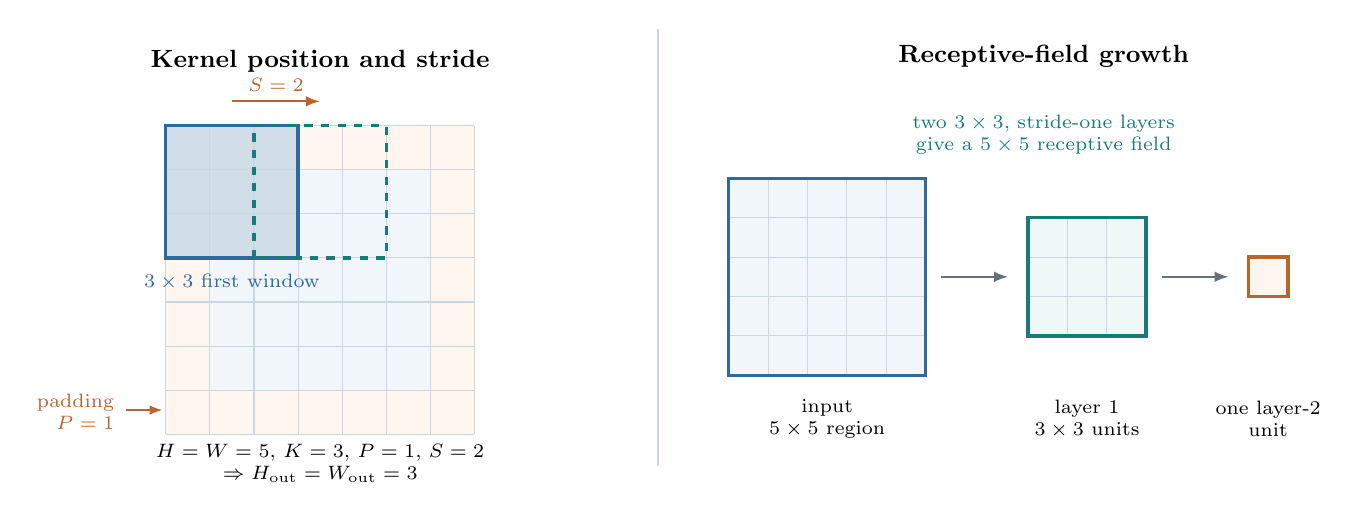
\begin{tikzpicture}[font=\scriptsize]
% Padding, kernel, and stride.
\begin{scope}[x=0.56cm,y=0.56cm]
  \fill[PaleOrange] (0,0) rectangle (7,7);
  \fill[PaleBlue] (1,1) rectangle (6,6);
  \fill[Blue!22] (0,4) rectangle (3,7);
  \foreach \x in {0,...,7} {\draw[Rule] (\x,0)--(\x,7);}
  \foreach \y in {0,...,7} {\draw[Rule] (0,\y)--(7,\y);}
  \draw[Blue,very thick] (0,4) rectangle (3,7);
  \draw[Teal,very thick,dashed] (2,4) rectangle (5,7);
  \draw[-{Latex[length=1.8mm]},Orange,thick]
    (1.5,7.55)--node[above] {$S=2$}(3.5,7.55);
  \node[Blue,align=center] at (1.5,3.45) {$3\times3$\ first window};
  \draw[-{Latex[length=1.6mm]},Orange]
    (-0.9,0.55)--(-0.08,0.55);
  \node[Orange,anchor=e,align=right] at (-0.95,0.55) {padding\\$P=1$};
  \node[font=\bfseries\small] at (3.5,8.45)
    {Kernel position and stride};
  \node[align=center] at (3.5,-0.65)
    {$H=W=5$, $K=3$, $P=1$, $S=2$\\
     $\Rightarrow H_{\mathrm{out}}=W_{\mathrm{out}}=3$};
\end{scope}

\draw[Rule,thick] (6.25,-0.4)--(6.25,5.15);

% Receptive-field growth through two stacked convolutions.
\begin{scope}[shift={(7.15,0.75)}]
  \node[font=\bfseries\small] at (4.0,4.05)
    {Receptive-field growth};

  \fill[PaleBlue] (0,0) rectangle (2.5,2.5);
  \foreach \x in {0,0.5,...,2.5} {\draw[Rule] (\x,0)--(\x,2.5);}
  \foreach \y in {0,0.5,...,2.5} {\draw[Rule] (0,\y)--(2.5,\y);}
  \draw[Blue,very thick] (0,0) rectangle (2.5,2.5);
  \node[align=center] at (1.25,-0.55) {input\\$5\times5$ region};

  \fill[PaleTeal] (3.8,0.5) rectangle (5.3,2.0);
  \foreach \x in {3.8,4.3,4.8,5.3} {\draw[Rule] (\x,0.5)--(\x,2.0);}
  \foreach \y in {0.5,1.0,1.5,2.0} {\draw[Rule] (3.8,\y)--(5.3,\y);}
  \draw[Teal,very thick] (3.8,0.5) rectangle (5.3,2.0);
  \node[align=center] at (4.55,-0.55) {layer 1\\$3\times3$ units};

  \fill[PaleOrange] (6.6,1.0) rectangle (7.1,1.5);
  \draw[Orange,very thick] (6.6,1.0) rectangle (7.1,1.5);
  \node[align=center] at (6.85,-0.55) {one layer-2\\unit};

  \draw[-{Latex[length=1.8mm]},Ink!70,thick] (2.7,1.25)--(3.55,1.25);
  \draw[-{Latex[length=1.8mm]},Ink!70,thick] (5.5,1.25)--(6.35,1.25);
  \node[align=center,Teal] at (4.0,3.05)
    {two $3\times3$, stride-one layers\\give a $5\times5$ receptive field};
\end{scope}
\end{tikzpicture}
\caption{Convolution geometry. On the left, padding enlarges the effective input and stride moves the kernel between sampled positions; the stated values produce a $3\times3$ output. On the right, one unit after two $3\times3$, stride-one convolutions depends on a $5\times5$ input region, even though each individual operation is local.}
\label{fig:convolution-geometry}
\end{figure}}

\newcommand{\LstmFlowFigure}{%
\begin{figure}[htbp]
\centering
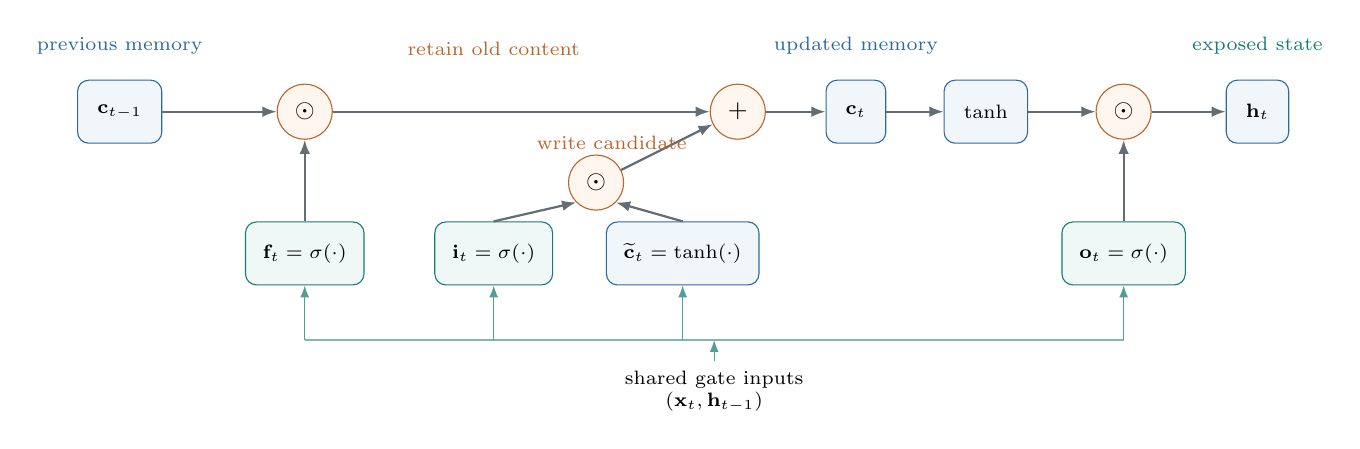
\begin{tikzpicture}[
  font=\scriptsize,
  state/.style={draw=Blue,rounded corners,fill=PaleBlue,minimum height=8mm,inner xsep=2.5mm},
  gate/.style={draw=Teal,rounded corners,fill=PaleTeal,minimum height=8mm,inner xsep=2.2mm},
  candidate/.style={draw=Blue,rounded corners,fill=PaleBlue,minimum height=8mm,inner xsep=2.2mm},
  op/.style={circle,draw=Orange,fill=PaleOrange,minimum size=7mm,inner sep=0pt,font=\small},
  arr/.style={-{Latex[length=1.8mm]},thick,color=Ink!72},
  inputarr/.style={-{Latex[length=1.5mm]},color=Teal!75}
]
\node[state] (cprev) at (0,1.55) {$\mathbf c_{t-1}$};
\node[op] (forgetmul) at (2.35,1.55) {$\odot$};
\node[op] (sum) at (7.85,1.55) {$+$};
\node[state] (ct) at (9.35,1.55) {$\mathbf c_t$};
\node[state] (tanhct) at (11.0,1.55) {$\tanh$};
\node[op] (outmul) at (12.75,1.55) {$\odot$};
\node[state] (ht) at (14.45,1.55) {$\mathbf h_t$};

\node[gate] (fgate) at (2.35,-0.25) {$\mathbf f_t=\sigma(\cdot)$};
\node[gate] (igate) at (4.75,-0.25) {$\mathbf i_t=\sigma(\cdot)$};
\node[candidate] (cand) at (7.15,-0.25)
  {$\widetilde{\mathbf c}_t=\tanh(\cdot)$};
\node[op] (writemul) at (6.05,0.65) {$\odot$};
\node[gate] (ogate) at (12.75,-0.25) {$\mathbf o_t=\sigma(\cdot)$};

\draw[arr] (cprev)--(forgetmul);
\draw[arr] (forgetmul)--(sum);
\draw[arr] (sum)--(ct);
\draw[arr] (ct)--(tanhct);
\draw[arr] (tanhct)--(outmul);
\draw[arr] (outmul)--(ht);
\draw[arr] (fgate)--(forgetmul);
\draw[arr] (igate.north)--(writemul.south west);
\draw[arr] (cand.north)--(writemul.south east);
\draw[arr] (writemul)--(sum);
\draw[arr] (ogate)--(outmul);

\node[align=center] (gateinput) at (7.55,-2.0)
  {shared gate inputs\\$(\mathbf x_t,\mathbf h_{t-1})$};
\draw[Teal!55,thick] (2.35,-1.35)--(12.75,-1.35);
\draw[inputarr] (gateinput)--(7.55,-1.35);
\draw[inputarr] (2.35,-1.35)--(fgate.south);
\draw[inputarr] (4.75,-1.35)--(igate.south);
\draw[inputarr] (7.15,-1.35)--(cand.south);
\draw[inputarr] (12.75,-1.35)--(ogate.south);

\node[Blue,above=2mm of cprev] {previous memory};
\node[Blue,above=2mm of ct] {updated memory};
\node[Teal,above=2mm of ht] {exposed state};
\node[Orange,align=center] at (4.75,2.35)
  {retain old content};
\node[Orange,align=center] at (6.25,1.15)
  {write candidate};
\end{tikzpicture}
\caption{Information flow in an LSTM cell. The forget and input branches form the additive update $\mathbf c_t=\mathbf f_t\odot\mathbf c_{t-1}+\mathbf i_t\odot\widetilde{\mathbf c}_t$; the output gate exposes $\mathbf h_t=\mathbf o_t\odot\tanh(\mathbf c_t)$. The gates and candidate all depend on $(\mathbf x_t,\mathbf h_{t-1})$.}
\label{fig:lstm-flow}
\end{figure}}

\newcommand{\KmeansIterationElbowFigure}{%
\begin{figure}[htbp]
\centering
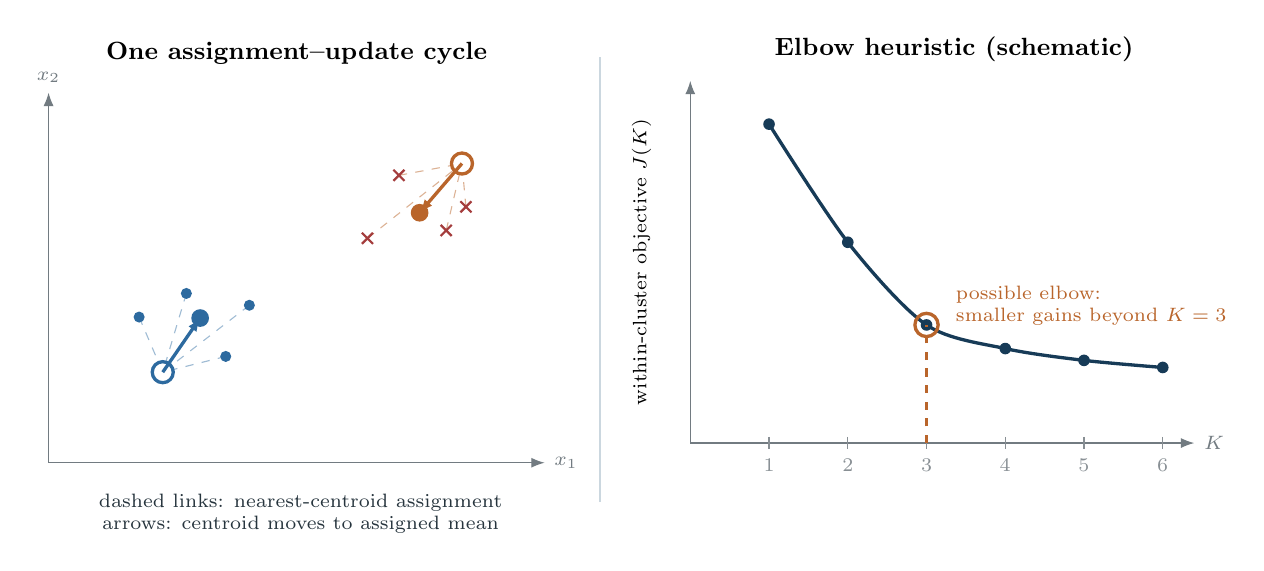
\begin{tikzpicture}[font=\scriptsize]
% Assignment and centroid update.
\begin{scope}
  \draw[-{Latex[length=1.7mm]},Ink!65] (0,0)--(6.3,0) node[right] {$x_1$};
  \draw[-{Latex[length=1.7mm]},Ink!65] (0,0)--(0,4.7) node[above] {$x_2$};

  \coordinate (oldone) at (1.45,1.15);
  \coordinate (newone) at (1.925,1.8375);
  \coordinate (oldtwo) at (5.25,3.80);
  \coordinate (newtwo) at (4.7125,3.175);

  \foreach \p in {(1.15,1.85),(1.75,2.15),(2.25,1.35),(2.55,2.00)} {
    \draw[Blue!45,dashed] \p--(oldone);
    \fill[Blue] \p circle (2pt);
  }
  \foreach \p in {(4.05,2.85),(4.45,3.65),(5.05,2.95),(5.30,3.25)} {
    \draw[Orange!50,dashed] \p--(oldtwo);
    \draw[Red,thick] \p ++(-2pt,-2pt)--++(4pt,4pt)
      \p ++(-2pt,2pt)--++(4pt,-4pt);
  }

  \draw[Blue,very thick,fill=white] (oldone) circle (3.8pt);
  \fill[Blue] (newone) circle (3.2pt);
  \draw[Orange,very thick,fill=white] (oldtwo) circle (3.8pt);
  \fill[Orange] (newtwo) circle (3.2pt);
  \draw[-{Latex[length=1.7mm]},Blue,very thick] (oldone)--(newone);
  \draw[-{Latex[length=1.7mm]},Orange,very thick] (oldtwo)--(newtwo);

  \node[font=\bfseries\small] at (3.15,5.2)
    {One assignment--update cycle};
  \node[align=center,Ink] at (3.2,-0.65)
    {dashed links: nearest-centroid assignment\\
     arrows: centroid moves to assigned mean};
\end{scope}

\draw[Rule,thick] (7.0,-0.5)--(7.0,5.15);

% Schematic elbow curve.
\begin{scope}[shift={(8.15,0.25)}]
  \draw[-{Latex[length=1.7mm]},Ink!65] (0,0)--(6.4,0) node[right] {$K$};
  \draw[-{Latex[length=1.7mm]},Ink!65] (0,0)--(0,4.6);
  \node[rotate=90] at (-0.62,2.30) {within-cluster objective $J(K)$};
  \foreach \k in {1,...,6} {
    \draw[Ink!55] (\k,0.08)--(\k,-0.08) node[below] {\k};
  }
  \draw[Navy,very thick]
    plot[smooth] coordinates {(1,4.05) (2,2.55) (3,1.50) (4,1.20) (5,1.05) (6,0.96)};
  \foreach \p in {(1,4.05),(2,2.55),(3,1.50),(4,1.20),(5,1.05),(6,0.96)}
    \fill[Navy] \p circle (2.1pt);
  \draw[Orange,dashed,thick] (3,0)--(3,1.50);
  \draw[Orange,very thick] (3,1.50) circle (4.2pt);
  \node[Orange,anchor=west,align=left] at (3.25,1.75)
    {possible elbow:\\smaller gains beyond $K=3$};
  \node[font=\bfseries\small] at (3.35,5.0)
    {Elbow heuristic (schematic)};
\end{scope}
\end{tikzpicture}
\caption{K-means alternates between assigning each sample to its nearest current centroid and replacing each centroid by its assigned mean; each step does not increase the objective. The elbow plot compares the final objective across values of $K$. A visible bend can guide model selection, but a smooth curve does not determine a unique $K$.}
\label{fig:kmeans-iteration-elbow}
\end{figure}}

\newcommand{\ActivationCouplingFigure}{%
\begin{figure}[htbp]
\centering
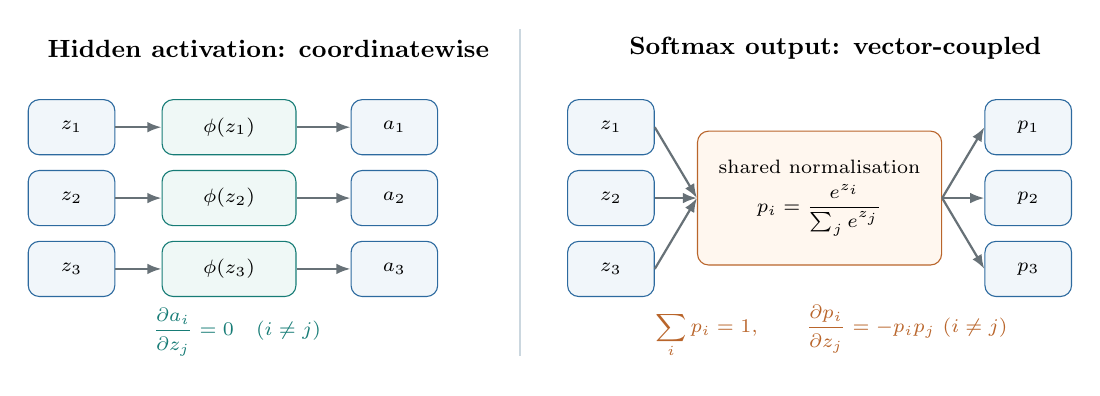
\begin{tikzpicture}[
  font=\scriptsize,
  value/.style={draw=Blue,rounded corners,fill=PaleBlue,
    minimum width=11mm,minimum height=7mm,inner sep=1.5mm},
  activated/.style={draw=Teal,rounded corners,fill=PaleTeal,
    minimum width=17mm,minimum height=7mm,inner sep=1.5mm},
  normalise/.style={draw=Orange,rounded corners,fill=PaleOrange,
    minimum width=31mm,minimum height=17mm,align=center,inner sep=2mm},
  arr/.style={-{Latex[length=1.8mm]},thick,color=Ink!70}
]
% Elementwise hidden activation.
\node[font=\small\bfseries] at (3.05,3.45)
  {Hidden activation: coordinatewise};
\foreach \i/\y in {1/2.45,2/1.55,3/0.65} {
  \node[value] (hz\i) at (0.55,\y) {$z_{\i}$};
  \node[activated] (hphi\i) at (2.55,\y) {$\phi(z_{\i})$};
  \node[value] (ha\i) at (4.65,\y) {$a_{\i}$};
  \draw[arr] (hz\i)--(hphi\i);
  \draw[arr] (hphi\i)--(ha\i);
}
\node[align=center,color=Teal] at (2.65,-0.15)
  {$\displaystyle \frac{\partial a_i}{\partial z_j}=0\quad(i\ne j)$};

\draw[Rule,thick] (6.25,-0.45)--(6.25,3.70);

% Vector-coupled Softmax output.
\begin{scope}[xshift=7.05cm]
  \node[font=\small\bfseries] at (3.20,3.45)
    {Softmax output: vector-coupled};
  \node[normalise] (snorm) at (3.00,1.55)
    {shared normalisation\\[1mm]
     $\displaystyle p_i=\frac{e^{z_i}}{\sum_j e^{z_j}}$};
  \foreach \i/\y in {1/2.45,2/1.55,3/0.65} {
    \node[value] (sz\i) at (0.35,\y) {$z_{\i}$};
    \node[value] (sp\i) at (5.65,\y) {$p_{\i}$};
    \draw[arr] (sz\i.east)--(snorm.west);
    \draw[arr] (snorm.east)--(sp\i.west);
  }
  \node[align=center,color=Orange] at (3.15,-0.15)
    {$\displaystyle \sum_i p_i=1,\qquad
      \frac{\partial p_i}{\partial z_j}=-p_i p_j\ (i\ne j)$};
\end{scope}
\end{tikzpicture}
\caption{Hidden-layer activations such as ReLU act coordinate by coordinate: changing $z_j$ directly changes only $a_j$. Softmax uses a shared denominator, so changing one logit generally changes every class probability.}
\label{fig:activation-coupling}
\end{figure}}

\newcommand{\AutoencoderManifoldFigure}{%
\begin{figure}[htbp]
\centering
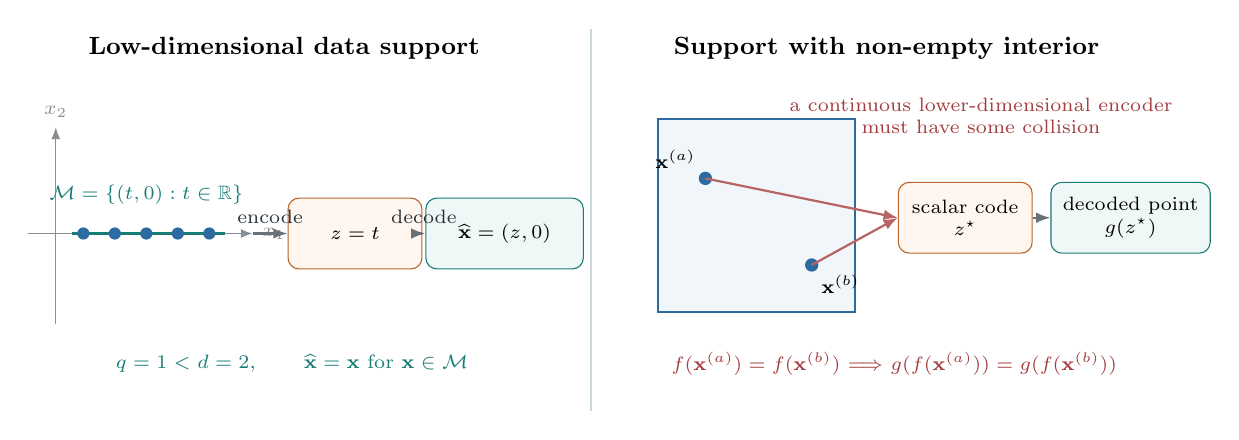
\begin{tikzpicture}[
  font=\scriptsize,
  code/.style={draw=Orange,rounded corners,fill=PaleOrange,
    minimum width=17mm,minimum height=9mm,align=center,inner sep=1.5mm},
  recon/.style={draw=Teal,rounded corners,fill=PaleTeal,
    minimum width=20mm,minimum height=9mm,align=center,inner sep=1.5mm},
  arr/.style={-{Latex[length=1.8mm]},thick,color=Ink!70},
  collision/.style={-{Latex[length=1.8mm]},thick,color=Red!80}
]
% Exact reconstruction on lower-dimensional support.
\node[font=\small\bfseries] at (3.45,4.55)
  {Low-dimensional data support};
\draw[-{Latex[length=1.5mm]},Ink!55] (0.20,2.20)--(3.05,2.20)
  node[right] {$x_1$};
\draw[-{Latex[length=1.5mm]},Ink!55] (0.55,1.05)--(0.55,3.55)
  node[above] {$x_2$};
\draw[Teal,very thick] (0.75,2.20)--(2.70,2.20);
\foreach \x in {0.90,1.30,1.70,2.10,2.50}
  \fill[Blue] (\x,2.20) circle (2.2pt);
\node[Teal,above] at (1.70,2.45)
  {$\mathcal M=\{(t,0):t\in\mathbb R\}$};
\node[code] (exactcode) at (4.35,2.20) {$z=t$};
\node[recon] (exactrecon) at (6.25,2.20)
  {$\widehat{\mathbf x}=(z,0)$};
\draw[arr] (3.05,2.20)--node[above,color=Ink]{encode}(exactcode);
\draw[arr] (exactcode)--node[above,color=Ink]{decode}(exactrecon);
\node[align=center,color=Teal] at (3.55,0.55)
  {$q=1<d=2,\qquad \widehat{\mathbf x}=\mathbf x$
   for $\mathbf x\in\mathcal M$};

\draw[Rule,thick] (7.35,-0.05)--(7.35,4.80);

% Collision on full-dimensional support.
\begin{scope}[xshift=8.05cm]
  \node[font=\small\bfseries] at (3.05,4.55)
    {Support with non-empty interior};
  \fill[PaleBlue] (0.15,1.20) rectangle (2.65,3.65);
  \draw[Blue,thick] (0.15,1.20) rectangle (2.65,3.65);
  \coordinate (xa) at (0.75,2.90);
  \coordinate (xb) at (2.10,1.80);
  \fill[Blue] (xa) circle (2.4pt);
  \fill[Blue] (xb) circle (2.4pt);
  \node[anchor=south east] at (xa) {$\mathbf x^{(a)}$};
  \node[anchor=north west] at (xb) {$\mathbf x^{(b)}$};
  \node[code] (sharedcode) at (4.05,2.40) {scalar code\\$z^\star$};
  \node[recon] (sharedrecon) at (6.15,2.40)
    {decoded point\\$g(z^\star)$};
  \draw[collision] (xa)--(sharedcode.west);
  \draw[collision] (xb)--(sharedcode.west);
  \draw[arr] (sharedcode)--(sharedrecon);
  \node[Red,align=center] at (4.25,3.70)
    {a continuous lower-dimensional encoder\\must have some collision};
  \node[align=center,color=Red] at (3.15,0.55)
    {$f(\mathbf x^{(a)})=f(\mathbf x^{(b)})$
     $\Longrightarrow$
     $g(f(\mathbf x^{(a)}))=g(f(\mathbf x^{(b)}))$};
\end{scope}
\end{tikzpicture}
\caption{An undercomplete code need not lose information. For $\mathcal M=\{(t,0):t\in\mathbb R\}\subset\mathbb R^2$, the maps $f(t,0)=t$ and $g(t)=(t,0)$ reconstruct every point exactly with $q=1<d=2$. By contrast, if the data support contains a full-dimensional open set and the encoder is continuous, a lower-dimensional encoder cannot be injective on that support. Bottleneck width constrains capacity but does not by itself determine information loss or representation quality.}
\label{fig:autoencoder-manifold}
\end{figure}}


\section{From the Perceptron to Multilayer Networks}
\label{sec:mlp}

A linear model reduces an input to a score and predicts from that score. A neural network retains the affine computation but composes several layers, placing a nonlinear function between successive affine transformations.

\subsection{The perceptron as a single neuron}

For binary labels $y\in\{-1,+1\}$, the perceptron computes
\[
    a(\mathbf{x})=\mathbf{w}^{\mathsf T}\mathbf{x}+b
\]
and applies a sign activation:
\[
    \widehat{y}=\operatorname{sign}\!\left(a(\mathbf{x})\right).
\]
Section~\ref{sec:perceptron} gives the update rule, loss, and convergence
condition. As a network unit, the perceptron exposes the limitation that
motivates hidden layers: a sign applied to one affine score still produces a
linear decision boundary.

\subsection{Multilayer perceptrons}

In a multilayer perceptron (MLP), each hidden layer \(l\) first applies an affine transformation and then an elementwise activation function:
\begin{align}
    \mathbf{z}^{(l)}
    &=\mathbf{W}^{(l)}\mathbf{a}^{(l-1)}+\mathbf{b}^{(l)},
    \label{eq:mlp-affine}\\
    \mathbf{a}^{(l)}
    &=\phi^{(l)}\!\left(\mathbf{z}^{(l)}\right),
    \label{eq:mlp-activation}
\end{align}
with \(\mathbf{a}^{(0)}=\mathbf{x}\). The vector \(\mathbf{z}^{(l)}\) contains the pre-activations of layer \(l\), and \(\mathbf{a}^{(l)}\) is its output.

The nonlinear activation is essential. If every layer is affine, then two successive layers can still be written as one affine map:
\[
    \mathbf{W}^{(2)}
    \bigl(\mathbf{W}^{(1)}\mathbf{x}+\mathbf{b}^{(1)}\bigr)
    +\mathbf{b}^{(2)}
    =\widetilde{\mathbf{W}}\mathbf{x}+\widetilde{\mathbf{b}}.
\]
Adding affine layers alone does not enlarge the class of functions represented by the model.

On a compact input domain, a one-hidden-layer network with sufficient width and
a suitable non-polynomial activation can approximate any continuous target
function arbitrarily closely. This universal-approximation result is a statement
about representational capacity; it does not guarantee an efficient width,
successful optimisation, or generalisation beyond the training distribution.

Common activation functions and their derivatives are
\begin{align*}
    \operatorname{sigmoid}(z)
    &=\sigma(z)=\frac{1}{1+e^{-z}},
    & \sigma'(z)&=\sigma(z)\bigl(1-\sigma(z)\bigr),\\
    \tanh(z)
    &=\frac{e^z-e^{-z}}{e^z+e^{-z}},
    & \frac{\mathrm{d}}{\mathrm{d}z}\tanh(z)&=1-\tanh^2(z),\\
    \operatorname{ReLU}(z)
    &=\max\{0,z\},
    & \operatorname{ReLU}'(z)&=
    \begin{cases}
        0,&z<0,\\
        1,&z>0.
    \end{cases}
\end{align*}
ReLU is not differentiable at \(z=0\); implementations select a conventional subgradient there, commonly zero. Sigmoid and \(\tanh\) are smooth but saturate for inputs of large magnitude. ReLU has derivative one on the positive half-line and zero on the negative half-line.

\subsection{Output layers and loss functions}

The output transformation and loss function must match the prediction task.

\paragraph{Regression.}
For a real-valued target, a linear output \(\widehat{\mathbf{y}}=\mathbf{z}\) can be paired with squared error:
\[
    \mathcal{L}_{\mathrm{MSE}}
    =\frac{1}{2}\left\lVert
    \widehat{\mathbf{y}}-\mathbf{y}
    \right\rVert_2^2.
\]
The factor \(1/2\) simplifies the derivative and does not change the minimiser.

\paragraph{Binary classification.}
Let \(p=\sigma(z)\) denote the probability of the positive class and let \(y\in\{0,1\}\). The binary cross-entropy is
\[
    \mathcal{L}_{\mathrm{BCE}}
    =-y\log p-(1-y)\log(1-p).
\]

\paragraph{Mutually exclusive multiclass classification.}
If each sample belongs to exactly one of \(K\) classes, the output layer uses Softmax:
\begin{equation}
    p_k
    =\frac{e^{z_k}}{\sum_{j=1}^{K}e^{z_j}},
    \qquad k=1,\ldots,K.
    \label{eq:softmax}
\end{equation}
The resulting values satisfy \(p_k\geq0\) and \(\sum_k p_k=1\). Stable implementations set \(m=\max_j z_j\) and evaluate Softmax using \(z_k-m\). This shift leaves the probabilities unchanged and prevents overflow in the exponential.

For a one-hot target, or more generally for \(y_k\geq0\) and \(\sum_k y_k=1\), the multiclass cross-entropy is
\begin{equation}
    \mathcal{L}_{\mathrm{CE}}
    =-\sum_{k=1}^{K}y_k\log p_k.
    \label{eq:cross-entropy}
\end{equation}

\paragraph{Multilabel classification.}
When several labels may be present simultaneously, the classes should not share one softmax normalisation. The model instead computes \(p_k=\sigma(z_k)\) independently for each class and sums the \(K\) binary cross-entropies.

\ActivationCouplingFigure

\subsection{The Softmax--cross-entropy gradient}

The Jacobian of Softmax is
\begin{equation}
    \frac{\partial p_k}{\partial z_j}
    =p_k\bigl(\mathbb{I}[k=j]-p_j\bigr),
    \label{eq:softmax-jacobian}
\end{equation}
where \(\mathbb{I}[k=j]\) equals one when \(k=j\) and zero otherwise. Substitution into the derivative of cross-entropy gives
\begin{align*}
    \frac{\partial\mathcal{L}_{\mathrm{CE}}}{\partial z_j}
    &=-\sum_{k=1}^{K}
      \frac{y_k}{p_k}
      \frac{\partial p_k}{\partial z_j}\\
    &=-\sum_{k=1}^{K}y_k
      \bigl(\mathbb{I}[k=j]-p_j\bigr)\\
    &=p_j\sum_{k=1}^{K}y_k-y_j\\
    &=p_j-y_j.
\end{align*}
Thus,
\begin{equation}
    \nabla_{\mathbf{z}}\mathcal{L}_{\mathrm{CE}}
    =\mathbf{p}-\mathbf{y}.
    \label{eq:softmax-ce-gradient}
\end{equation}
The gradient $\mathbf p-\mathbf y$ results from the composition of softmax and cross-entropy, rather than from softmax alone.

\subsection{Forward and backward computation in a two-layer network}

Consider a \(K\)-class network with one hidden layer of width \(m\):
\begin{align}
    \mathbf{z}^{(1)}
    &=\mathbf{W}^{(1)}\mathbf{x}+\mathbf{b}^{(1)},
    & \mathbf{W}^{(1)}&\in\mathbb{R}^{m\times d},
    \label{eq:two-layer-z1}\\
    \mathbf{h}
    &=\phi\!\left(\mathbf{z}^{(1)}\right),
    & \mathbf{h}&\in\mathbb{R}^{m},
    \label{eq:two-layer-h}\\
    \mathbf{z}^{(2)}
    &=\mathbf{W}^{(2)}\mathbf{h}+\mathbf{b}^{(2)},
    & \mathbf{W}^{(2)}&\in\mathbb{R}^{K\times m},
    \label{eq:two-layer-z2}\\
    \mathbf{p}
    &=\operatorname{softmax}\!\left(\mathbf{z}^{(2)}\right),
    & \mathcal{L}&=-\sum_{k=1}^{K}y_k\log p_k.
    \label{eq:two-layer-output}
\end{align}

\BackpropFigure

Backpropagation applies the chain rule in reverse computational order. The output error signal follows from Equation~\eqref{eq:softmax-ce-gradient}:
\[
    \boldsymbol{\delta}^{(2)}
    :=\frac{\partial\mathcal{L}}{\partial\mathbf{z}^{(2)}}
    =\mathbf{p}-\mathbf{y}.
\]
Since \(\mathbf{z}^{(2)}=\mathbf{W}^{(2)}\mathbf{h}+\mathbf{b}^{(2)}\), the output-layer gradients are
\begin{align}
    \frac{\partial\mathcal{L}}{\partial\mathbf{W}^{(2)}}
    &=\boldsymbol{\delta}^{(2)}\mathbf{h}^{\mathsf T},
    \label{eq:grad-w2}\\
    \frac{\partial\mathcal{L}}{\partial\mathbf{b}^{(2)}}
    &=\boldsymbol{\delta}^{(2)}.
    \label{eq:grad-b2}
\end{align}
The matrix in Equation~\eqref{eq:grad-w2} has shape \(K\times m\), matching \(\mathbf{W}^{(2)}\).

The gradient with respect to the hidden representation is
\[
    \frac{\partial\mathcal{L}}{\partial\mathbf{h}}
    =\left(\mathbf{W}^{(2)}\right)^{\mathsf T}
      \boldsymbol{\delta}^{(2)}.
\]
Passing this gradient through the elementwise activation gives
\begin{equation}
    \boldsymbol{\delta}^{(1)}
    :=\frac{\partial\mathcal{L}}{\partial\mathbf{z}^{(1)}}
    =\left[
      \left(\mathbf{W}^{(2)}\right)^{\mathsf T}
      \boldsymbol{\delta}^{(2)}
    \right]
    \odot
    \phi'\!\left(\mathbf{z}^{(1)}\right),
    \label{eq:delta-one}
\end{equation}
where \(\odot\) denotes elementwise multiplication. The first-layer gradients are
\begin{align}
    \frac{\partial\mathcal{L}}{\partial\mathbf{W}^{(1)}}
    &=\boldsymbol{\delta}^{(1)}\mathbf{x}^{\mathsf T},
    \label{eq:grad-w1}\\
    \frac{\partial\mathcal{L}}{\partial\mathbf{b}^{(1)}}
    &=\boldsymbol{\delta}^{(1)}.
    \label{eq:grad-b1}
\end{align}
For a mini-batch of size \(B\), the usual update averages the sample gradients:
\[
    \mathbf{W}^{(l)}
    \leftarrow
    \mathbf{W}^{(l)}
    -\eta\frac{1}{B}
    \sum_{i=1}^{B}
    \frac{\partial\mathcal{L}_i}
         {\partial\mathbf{W}^{(l)}}.
\]

The same recurrence extends to any number of layers. For
\(\boldsymbol{\delta}^{(l)}=
\partial\mathcal{L}/\partial\mathbf{z}^{(l)}\),
\begin{align}
    \boldsymbol{\delta}^{(l)}
    &=\left[
      \left(\mathbf{W}^{(l+1)}\right)^{\mathsf T}
      \boldsymbol{\delta}^{(l+1)}
    \right]
    \odot
    \phi^{(l)\prime}\!\left(\mathbf{z}^{(l)}\right),
    \label{eq:general-backprop-delta}\\
    \frac{\partial\mathcal{L}}{\partial\mathbf{W}^{(l)}}
    &=\boldsymbol{\delta}^{(l)}
      \left(\mathbf{a}^{(l-1)}\right)^{\mathsf T},
    \qquad
    \frac{\partial\mathcal{L}}{\partial\mathbf{b}^{(l)}}
    =\boldsymbol{\delta}^{(l)}.
    \label{eq:general-backprop-parameter}
\end{align}
Backpropagation evaluates the chain rule efficiently by caching forward-pass intermediates and reusing them during the reverse pass.

\subsection{Saturation and vanishing gradients}

Gradients in a deep network contain products of many Jacobians. For a network with \(L\) elementwise activation layers,
\[
    \frac{\partial\mathbf{a}^{(L)}}
         {\partial\mathbf{a}^{(0)}}
    =\mathbf{D}^{(L)}\mathbf{W}^{(L)}
     \cdots
     \mathbf{D}^{(1)}\mathbf{W}^{(1)},
    \qquad
    \mathbf{D}^{(l)}
    =\operatorname{diag}\!\left(
      \phi^{(l)\prime}(\mathbf{z}^{(l)})
    \right).
\]
If the norms of most factors are below one, the product decays rapidly with depth and gradients near the input approach zero. Repeated factors with norms above one can instead produce exploding gradients.

Sigmoid satisfies
\[
    0<\sigma'(z)\leq\frac{1}{4},
\]
and its derivative approaches zero as \(|z|\) grows. The derivative of \(\tanh\) also approaches zero in its saturated regions. ReLU reduces this source of decay on its positive half-line, where its derivative is one, but has zero derivative on its negative half-line. A unit that remains negative may therefore stop updating. ReLU neither has derivative one everywhere nor guarantees that gradients cannot vanish.

Initialisation should keep activation and gradient scales from changing too rapidly across layers. Xavier initialisation is commonly paired with approximately symmetric activations such as \(\tanh\), while He initialisation is commonly paired with ReLU. Recurrent networks face the same issue across time steps; gated state updates help control gradient flow over long sequences.


\section{Convolutional and Recurrent Networks}
\label{sec:cnn-rnn}

Fully connected layers do not encode spatial or temporal structure. Nearby pixels in an image are often related, while a position in a sequence may depend on earlier positions. Convolutional networks use local connectivity and spatial parameter sharing. Recurrent networks share parameters across time and propagate a hidden state along the sequence.

\subsection{A convolutional layer computes cross-correlation}

Let the input be
\[
    \mathbf{X}\in
    \mathbb{R}^{H\times W\times C_{\mathrm{in}}}.
\]
For a kernel of spatial size \(K_h\times K_w\), with
\(C_{\mathrm{in}}\) input channels and \(C_{\mathrm{out}}\) output channels, the complete weight tensor has shape
\[
    \mathbf{K}\in
    \mathbb{R}^{K_h\times K_w\times
    C_{\mathrm{in}}\times C_{\mathrm{out}}}.
\]
The pre-activation at spatial location \((i,j)\) and output channel \(o\) is
\begin{equation}
    Z_{i,j,o}
    =b_o+
    \sum_{u=0}^{K_h-1}
    \sum_{v=0}^{K_w-1}
    \sum_{c=1}^{C_{\mathrm{in}}}
    K_{u,v,c,o}\,
    \widetilde{X}_{iS_h+u,\,jS_w+v,\,c},
    \label{eq:cnn-cross-correlation}
\end{equation}
where \(S_h,S_w\) are the strides and \(\widetilde{\mathbf{X}}\) is the padded input. Equation~\eqref{eq:cnn-cross-correlation} does not reverse the kernel horizontally and vertically, so the operation is formally cross-correlation. Machine-learning software and texts conventionally call it convolution.

Each output channel has one scalar bias \(b_o\). One output channel corresponds to a three-dimensional filter spanning all input channels, not a filter applied to only one channel. The number of parameters is
\begin{equation}
    K_hK_wC_{\mathrm{in}}C_{\mathrm{out}}
    +C_{\mathrm{out}}.
    \label{eq:cnn-parameter-count}
\end{equation}
This count does not grow with the input height or width because the same kernel parameters are reused at every spatial position.

\subsection{Kernel size, stride, padding, and output size}

With padding \(P_h,P_w\) and strides \(S_h,S_w\), the output dimensions are
\begin{align}
    H_{\mathrm{out}}
    &=\left\lfloor
      \frac{H+2P_h-K_h}{S_h}
      \right\rfloor+1,
    \label{eq:cnn-height}\\
    W_{\mathrm{out}}
    &=\left\lfloor
      \frac{W+2P_w-K_w}{S_w}
      \right\rfloor+1.
    \label{eq:cnn-width}
\end{align}
These expressions assume dilation one. Kernel size specifies the local receptive field of one operation; stride specifies the displacement between operations; padding adds rows and columns around the boundary. For an odd-sized kernel and unit stride, choosing
\[
    P_h=\frac{K_h-1}{2},
    \qquad
    P_w=\frac{K_w-1}{2}
\]
preserves the spatial dimensions.

For example, a \(32\times32\) input passed through a \(3\times3\) kernel with padding one and stride one remains \(32\times32\). If only the stride changes to two, then
\[
    H_{\mathrm{out}}
    =W_{\mathrm{out}}
    =\left\lfloor\frac{32+2-3}{2}\right\rfloor+1
    =16.
\]

\ConvolutionGeometryFigure

\subsection{Pooling}

Pooling aggregates values within a local window. Max pooling returns the largest value, while average pooling returns the mean. The window size and stride determine the output size through the same calculation as Equations~\eqref{eq:cnn-height}--\eqref{eq:cnn-width}, using the pooling-window parameters.

Standard pooling has no learned parameters. During backpropagation, max pooling routes the gradient only to a location that attained the maximum in the forward pass; average pooling distributes the gradient equally across the window. Pooling reduces spatial resolution and subsequent computation, but discards precise positional information. A strided convolution can instead learn the downsampling operation.

\subsection{Recurrent neural networks}

Given a sequence \(\mathbf{x}_1,\ldots,\mathbf{x}_T\), a basic recurrent neural network (RNN) updates its hidden state sequentially:
\begin{align}
    \mathbf{a}_t
    &=\mathbf{W}_x\mathbf{x}_t
      +\mathbf{U}\mathbf{h}_{t-1}
      +\mathbf{b},
    \label{eq:rnn-preactivation}\\
    \mathbf{h}_t
    &=\phi(\mathbf{a}_t),
    \label{eq:rnn-state}\\
    \mathbf{q}_t
    &=\mathbf{W}_y\mathbf{h}_t+\mathbf{b}_y.
    \label{eq:rnn-output}
\end{align}
The vector $\mathbf q_t$ contains the output logits. The matrices \(\mathbf{W}_x,\mathbf{U},\mathbf{W}_y\) are shared across all time steps. An unrolled network appears to contain \(T\) cells, but every cell refers to the same parameters. Its parameter count is therefore independent of sequence length.

The state \(\mathbf{h}_t\) carries information from earlier positions that is relevant to the current computation. A loss may be applied only at the final position or at every position. The latter case can be written as
\[
    \mathcal{L}=\sum_{t=1}^{T}\ell_t(\mathbf{q}_t).
\]

\subsection{Backpropagation through time}

Training an RNN requires backpropagation through time (BPTT). Define
\[
    \mathbf e_t
    :=\frac{\partial\ell_t}{\partial\mathbf q_t},
    \qquad
    \boldsymbol{\delta}_t
    :=\frac{\partial\mathcal{L}}{\partial\mathbf{a}_t},
    \qquad
    \boldsymbol{\delta}_{T+1}=\mathbf{0}.
\]
Working backwards from \(t=T\),
\begin{equation}
    \boldsymbol{\delta}_t
    =\left(
      \mathbf W_y^{\mathsf T}\mathbf e_t
      +\mathbf{U}^{\mathsf T}\boldsymbol{\delta}_{t+1}
    \right)
    \odot\phi'(\mathbf{a}_t).
    \label{eq:bptt-recurrence}
\end{equation}
The gradients of shared parameters sum the contributions from all time steps:
\begin{align}
    \frac{\partial\mathcal{L}}{\partial\mathbf{W}_x}
    &=\sum_{t=1}^{T}
      \boldsymbol{\delta}_t\mathbf{x}_t^{\mathsf T},
    \label{eq:bptt-wx}\\
    \frac{\partial\mathcal{L}}{\partial\mathbf{U}}
    &=\sum_{t=1}^{T}
      \boldsymbol{\delta}_t\mathbf{h}_{t-1}^{\mathsf T},
    \label{eq:bptt-u}\\
    \frac{\partial\mathcal{L}}{\partial\mathbf{b}}
    &=\sum_{t=1}^{T}\boldsymbol{\delta}_t.
    \label{eq:bptt-b}
    \\
    \frac{\partial\mathcal{L}}{\partial\mathbf{W}_y}
    &=\sum_{t=1}^{T}\mathbf e_t\mathbf h_t^{\mathsf T},
    &
    \frac{\partial\mathcal{L}}{\partial\mathbf b_y}
    &=\sum_{t=1}^{T}\mathbf e_t.
    \label{eq:bptt-output}
\end{align}
For a loss applied only at the final position, set $\mathbf e_t=\mathbf 0$ for $t<T$.

The influence of an early state on a later state contains a long product of recurrent Jacobians. In schematic form,
\[
    \frac{\partial\mathbf{h}_T}{\partial\mathbf{h}_t}
    =\prod_{s=t+1}^{T}
      \left[
      \operatorname{diag}\!\bigl(\phi'(\mathbf{a}_s)\bigr)
      \mathbf{U}
      \right],
\]
with the factors ordered by time. This product may decay to zero or grow rapidly, producing vanishing or exploding gradients. Gradient clipping limits exploding gradients but cannot restore gradients that have already vanished. Truncated BPTT propagates gradients through a finite time window, reducing computation and memory at the cost of discarding longer dependencies.

\subsection{Information flow in an LSTM}

A long short-term memory network (LSTM) introduces a cell state \(\mathbf{c}_t\) and gates that control retention, writing, and readout. One common parameterisation is
\begin{align}
    \mathbf{f}_t
    &=\sigma\!\left(
      \mathbf{W}_f\mathbf{x}_t
      +\mathbf{U}_f\mathbf{h}_{t-1}
      +\mathbf{b}_f
    \right),\\
    \mathbf{i}_t
    &=\sigma\!\left(
      \mathbf{W}_i\mathbf{x}_t
      +\mathbf{U}_i\mathbf{h}_{t-1}
      +\mathbf{b}_i
    \right),\\
    \widetilde{\mathbf{c}}_t
    &=\tanh\!\left(
      \mathbf{W}_c\mathbf{x}_t
      +\mathbf{U}_c\mathbf{h}_{t-1}
      +\mathbf{b}_c
    \right),\\
    \mathbf{c}_t
    &=\mathbf{f}_t\odot\mathbf{c}_{t-1}
      +\mathbf{i}_t\odot\widetilde{\mathbf{c}}_t,
    \label{eq:lstm-cell}\\
    \mathbf{o}_t
    &=\sigma\!\left(
      \mathbf{W}_o\mathbf{x}_t
      +\mathbf{U}_o\mathbf{h}_{t-1}
      +\mathbf{b}_o
    \right),\\
    \mathbf{h}_t
    &=\mathbf{o}_t\odot\tanh(\mathbf{c}_t).
    \label{eq:lstm-hidden}
\end{align}

\LstmFlowFigure

The forget gate \(\mathbf{f}_t\) controls retention of the previous cell state, the input gate \(\mathbf{i}_t\) controls writing of the candidate state, and the output gate \(\mathbf{o}_t\) controls how much of the cell state enters the hidden representation. Along the direct cell-state path in Equation~\eqref{eq:lstm-cell},
\[
    \frac{\partial\mathbf{c}_t}
         {\partial\mathbf{c}_{t-1}}
    =\operatorname{diag}(\mathbf{f}_t),
\]
when the gate dependence is held fixed. If the forget gate remains close to one, gradients can travel farther through the additive state update. This mechanism mitigates vanishing gradients but does not guarantee preservation of dependencies of arbitrary length.

\subsection{Information flow in a GRU}

A gated recurrent unit (GRU) has no separate cell state. The following convention lets larger \(\mathbf{z}_t\) write more of the candidate state:
\begin{align}
    \mathbf{r}_t
    &=\sigma\!\left(
      \mathbf{W}_r\mathbf{x}_t
      +\mathbf{U}_r\mathbf{h}_{t-1}
      +\mathbf{b}_r
    \right),\\
    \mathbf{z}_t
    &=\sigma\!\left(
      \mathbf{W}_z\mathbf{x}_t
      +\mathbf{U}_z\mathbf{h}_{t-1}
      +\mathbf{b}_z
    \right),\\
    \widetilde{\mathbf{h}}_t
    &=\tanh\!\left(
      \mathbf{W}_h\mathbf{x}_t
      +\mathbf{U}_h
       (\mathbf{r}_t\odot\mathbf{h}_{t-1})
      +\mathbf{b}_h
    \right),\\
    \mathbf{h}_t
    &=(\mathbf{1}-\mathbf{z}_t)
      \odot\mathbf{h}_{t-1}
      +\mathbf{z}_t\odot\widetilde{\mathbf{h}}_t.
    \label{eq:gru-update}
\end{align}
The reset gate \(\mathbf{r}_t\) controls how much of the previous state enters the candidate computation. The update gate \(\mathbf{z}_t\) interpolates between the previous state and the candidate. Some texts use the opposite convention for \(\mathbf{z}_t\); the state-update equation determines its meaning. A GRU has fewer gates and usually fewer parameters than an LSTM with the same hidden width.


\section{Unsupervised Learning and Autoencoders}
\label{sec:unsupervised}

Unsupervised objectives are defined directly on the inputs: $k$-means minimises within-cluster distance, whereas an autoencoder minimises reconstruction error. Neither objective necessarily recovers groups that coincide with downstream class labels.

\ArchitectureFigure

\subsection{The K-means objective}

Given samples \(\mathbf{x}_1,\ldots,\mathbf{x}_n\in\mathbb{R}^{d}\) and a chosen number of clusters \(K\), let \(c_i\in\{1,\ldots,K\}\) be the assignment of sample \(i\), and let \(\boldsymbol{\mu}_k\) be the centre of cluster \(k\). K-means minimises the within-cluster sum of squares
\begin{equation}
    J(\mathbf{c},\boldsymbol{\mu})
    =\sum_{i=1}^{n}
      \left\lVert
      \mathbf{x}_i-\boldsymbol{\mu}_{c_i}
      \right\rVert_2^2.
    \label{eq:kmeans-objective}
\end{equation}
The objective contains both discrete assignments and continuous centroids, so it is normally optimised by alternating between them.

With fixed centroids, each sample is assigned to its nearest centroid:
\begin{equation}
    c_i
    \leftarrow
    \operatorname*{arg\,min}_{k\in\{1,\ldots,K\}}
    \left\lVert
    \mathbf{x}_i-\boldsymbol{\mu}_k
    \right\rVert_2^2.
    \label{eq:kmeans-assignment}
\end{equation}
With fixed assignments, centroid \(k\) is updated to the mean of its assigned samples:
\begin{equation}
    \boldsymbol{\mu}_k
    \leftarrow
    \frac{1}{|C_k|}
    \sum_{i:c_i=k}\mathbf{x}_i,
    \qquad
    C_k=\{i:c_i=k\}.
    \label{eq:kmeans-centroid}
\end{equation}

\KmeansIterationElbowFigure

The mean minimises squared error within a fixed cluster. Both the assignment
step and the centroid step leave Equation~\eqref{eq:kmeans-objective} unchanged
or decrease it. Finite stabilisation follows when every assignment change
strictly decreases the objective, ties are resolved consistently, and empty
clusters are not reinitialised in a way that increases it. The endpoint is a
coordinate-wise fixed point, not necessarily a global optimum.

\subsection{Initialisation and scope}

The initial centroids affect the final solution. Selecting \(K\) data points
uniformly at random can place several initial centroids close together.
Multiple runs with different initialisations are therefore compared by their
final objective values; this reduces sensitivity to one poor initialisation but
does not guarantee a global optimum.

If a cluster receives no samples, Equation~\eqref{eq:kmeans-centroid} is undefined. An implementation may relocate that centroid to a sample with large current error or reinitialize it. Features should also be scaled before clustering when their numerical ranges differ, because squared Euclidean distance otherwise gives larger-scale features disproportionate influence.

K-means is most suitable for clusters that are approximately spherical, of comparable scale, and separable under Euclidean distance. It is sensitive to outliers and does not directly handle categorical variables or curved, nested clusters. The elbow method examines how \(J\) decreases as \(K\) grows; if the curve has no clear bend, it does not identify a unique number of clusters.

\subsection{The autoencoder objective}

An autoencoder consists of an encoder and a decoder:
\begin{align}
    \mathbf{z}
    &=f_{\boldsymbol{\theta}}(\mathbf{x}),
    \label{eq:ae-encoder}\\
    \widehat{\mathbf{x}}
    &=g_{\boldsymbol{\varphi}}(\mathbf{z}).
    \label{eq:ae-decoder}
\end{align}
The latent vector \(\mathbf{z}\) is an internal representation of the input. The parameters are learned through the reconstruction objective
\begin{equation}
    \min_{\boldsymbol{\theta},\boldsymbol{\varphi}}
    \frac{1}{n}\sum_{i=1}^{n}
    \ell\!\left(
      \mathbf{x}_i,
      g_{\boldsymbol{\varphi}}
      \bigl(f_{\boldsymbol{\theta}}(\mathbf{x}_i)\bigr)
    \right)
    +\Omega(\boldsymbol{\theta},\boldsymbol{\varphi}).
    \label{eq:ae-objective}
\end{equation}
Real-valued inputs are often trained with squared reconstruction error,
\[
    \ell(\mathbf{x},\widehat{\mathbf{x}})
    =\left\lVert
      \mathbf{x}-\widehat{\mathbf{x}}
    \right\rVert_2^2.
\]
Elementwise binary cross-entropy is appropriate when the input components have a Bernoulli interpretation. A Sigmoid output alone is not sufficient reason to assume this statistical model.

An autoencoder is undercomplete when
\[
    \dim(\mathbf{z})<\dim(\mathbf{x}).
\]
An undercomplete bottleneck limits representational capacity, but it does not by itself guarantee information loss on the data distribution. Data supported on a sufficiently low-dimensional set may still be reconstructed exactly. Under stronger conditions---for example, continuous encoder and decoder maps with data support containing a full-dimensional open set---an exact lower-dimensional code is impossible. If the latent dimension is at least the input dimension and the network has sufficient capacity, the model may approximate the identity map. In either case, low reconstruction error need not indicate a useful representation. Sparsity penalties, denoising objectives, and related regularisation mechanisms can discourage an identity-like solution, especially in an overcomplete model.

\AutoencoderManifoldFigure

\subsection{Linear autoencoders and PCA}

The relation between a linear autoencoder and principal component analysis holds only under specific conditions. Let \(\mathbf{X}\in\mathbb{R}^{n\times d}\) be a centred data matrix and let the bottleneck dimension be \(q<d\). With a linear encoder, a linear decoder, squared reconstruction error, and no bias, the objective is
\begin{equation}
    \min_{\mathbf{W}_e,\mathbf{W}_d}
    \left\lVert
      \mathbf{X}
      -\mathbf{X}\mathbf{W}_e\mathbf{W}_d
    \right\rVert_F^2,
    \qquad
    \mathbf{W}_e\in\mathbb{R}^{d\times q},
    \quad
    \mathbf{W}_d\in\mathbb{R}^{q\times d}.
    \label{eq:linear-ae}
\end{equation}
The optimal reconstruction subspace in Equation~\eqref{eq:linear-ae} is the subspace spanned by the first \(q\) principal components. Under the additional constraints
\[
    \mathbf{W}_d=\mathbf{W}_e^{\mathsf T},
    \qquad
    \mathbf{W}_e^{\mathsf T}\mathbf{W}_e=\mathbf{I},
\]
the reconstruction is the orthogonal projection
\[
    \widehat{\mathbf{X}}
    =\mathbf{X}\mathbf{W}_e\mathbf{W}_e^{\mathsf T},
\]
and the columns of an optimal \(\mathbf{W}_e\) can be chosen as the leading eigenvectors of the data covariance matrix.

Without the orthogonality constraint, latent coordinates are not unique. An invertible change of basis within the same principal subspace can yield the same reconstruction, so individual hidden units need not equal individual principal-component directions. Nonlinear activations, regularisation, or a different reconstruction loss also remove the equivalence with PCA.

\subsection{Sparse, deep, and convolutional autoencoders}

\paragraph{Sparse autoencoders.}
A sparse autoencoder may use a wide latent layer while requiring only a small
number of units to be active for each input. One option adds
$\lambda\lVert\mathbf z\rVert_1$ to the reconstruction objective, encouraging
the encoder to represent each input with relatively few active latent units.

\paragraph{Deep autoencoders.}
Both encoder and decoder may contain several nonlinear layers. Greater depth can represent nonlinear mappings, but the training problem is non-convex. A lower training reconstruction error does not imply better generalisation or a latent representation that is more suitable for a downstream task.

\paragraph{Convolutional autoencoders.}
For images, a convolutional encoder preserves local spatial structure and shares parameters across positions. The decoder commonly restores resolution through upsampling followed by convolution, or through transposed convolution. In the latter case, incompatible kernel and stride choices can create uneven overlap and grid artefacts.

\subsection{Limits of the compression interpretation}

A latent dimension smaller than the input dimension means only that each sample is represented internally by fewer numerical values. It does not determine the size of a compressed file, which also depends on numerical precision, quantisation, entropy coding, and the storage cost of the decoder.

The reconstruction loss determines which information is retained. Squared error favours directions with large numerical variation, which need not carry the semantics required by a classification task. Reconstruction error measures fidelity under the chosen data distribution and loss; it does not establish semantic class structure or a practical compression ratio.


\end{document}
